% The preamble has been dumped out as out/presentationpreamble.fmt file. You can recreate that file by
% xelatex -ini -jobname="pinholepreamble" -output-directory=out "&xelatex pinholepreamble.tex\dump"
% 
% To compile you need to load that binary file using -fmt option
% xelatex -fmt out/pinholepreamble.fmt -output-directory=out pinhole.tex
%\documentclass[10pt, compress]{beamer}
\usetheme{m}
 
 \usepackage{booktabs} % for better tables
 \usepackage{media9} % for includemedia i.e. videos
 \usepackage{xcolor} % for more colors
 \usepackage{hyperref} % for links
 \usepackage{cutwin} % text wrapped around figures
 \usepackage[backend=bibtex]{biblatex} % fancy citations
 \usepackage{ifthen}
 
\usepackage{tikz}
\usetikzlibrary{shadows,trees}
\usetikzlibrary{shapes,calc,backgrounds}
\usetikzlibrary{intersections}
\usepgfplotslibrary{dateplot}


%\tikzset{external/system call={xelatex -fmt out/pinholepreamble.fmt \tikzexternalcheckshellescape -shell-escape -halt-on-error -interaction=batchmode -jobname "\image" "\texsource"}}
%

% transparency
%\setbeamercovered{transparent=15}

\title{Light, pinholes and lenses: Cameras and computer imaging}
\date{\today}
\author{Chenliang Xu\\ Parker Koch\\ Vikas Dhiman\\ Jason J Corso}
\institute{University of Michigan}
\providecommand{\hl}[1]{{\color{red}{#1}}}

\begin{document}
\maketitle

\section{Modern Cameras}
\begin{frame}{Modern cameras}
    \includemedia[label=high-fps-camera,
      width=\linewidth,height=0.5\linewidth, % 16:9
      activate=pageopen,
      addresource=media/slowmolab.mp4,
      flashvars={
        source=media/bullet-time.mp4
        &loop=false             % loop video
        &scaleMode=letterbox   % preserve aspect ratio while scaling the video
      }
    ]{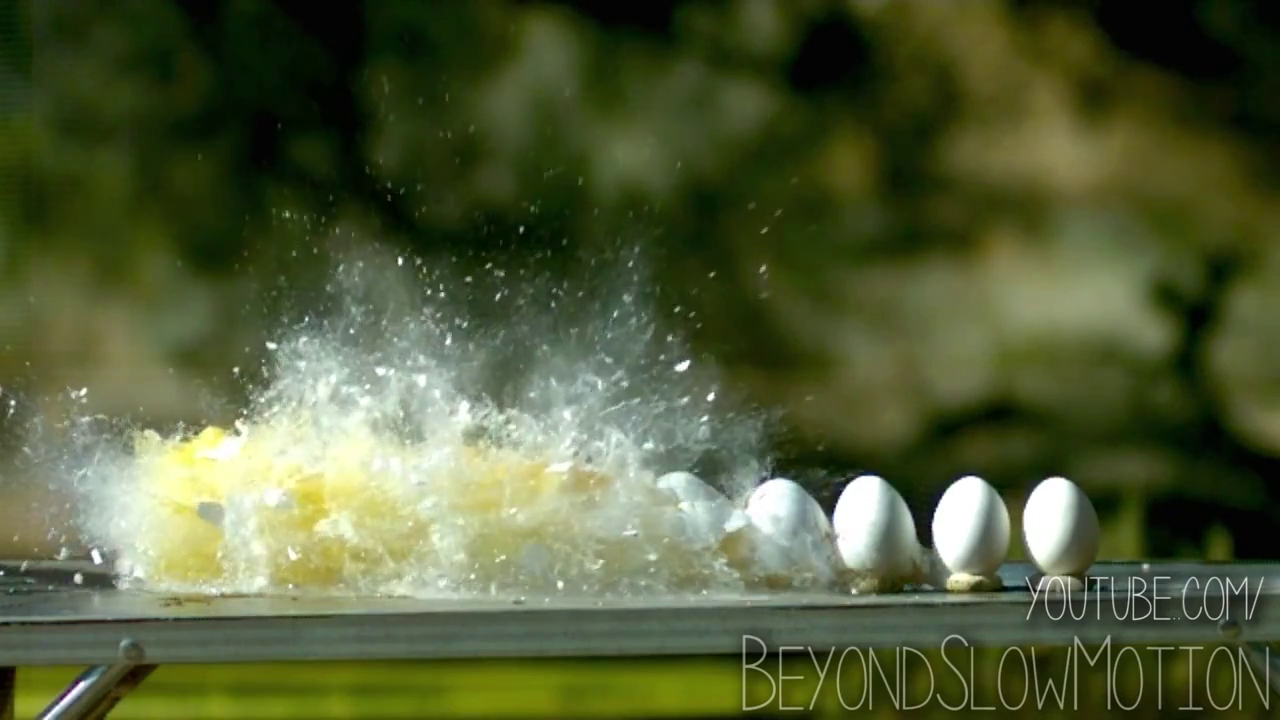
\includegraphics[width=\textwidth]{media/bullet-time.png}}{VPlayer.swf}
\end{frame}

\note{
  \hl{These notes can be disabled by removing notes option in the file pinholepreamble.tex}

  {Purpose: convey that modern cameras are powerful and complicated but the basic underlying principles remain the same.}
}

\begin{frame}{Modern cameras}
    \includemedia[label=matrix-bullet-time-shot,
      width=\linewidth,height=0.6\linewidth, % 16:9
      activate=pageopen,
      addresource=media/bullet-time-shot.mp4,
      flashvars={
        source=media/bullet-time-shot.mp4
        &loop=false             % loop video
        &scaleMode=letterbox   % preserve aspect ratio while scaling the video
      }
    ]{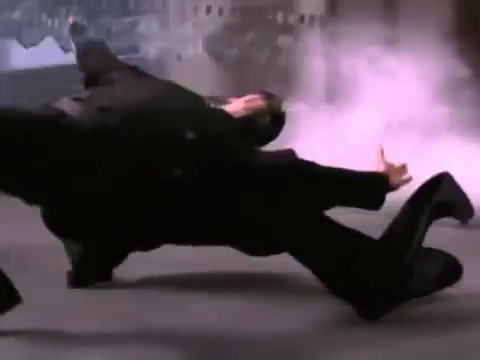
\includegraphics[width=\textwidth]{media/bullet-time-shot.png}}{VPlayer.swf}
\end{frame}

\section{About Light}
\begin{frame}{How do we see things?}
  
  \begin{tikzpicture}[scale=0.5]
    \path [use as bounding box] (-4,0) rectangle (11,13);
    \node [anchor=south](tree) at (0,0) {
\includegraphics[width=7cm]{media/tree.png}};
    \node [anchor=south] (boy) at (10,1) {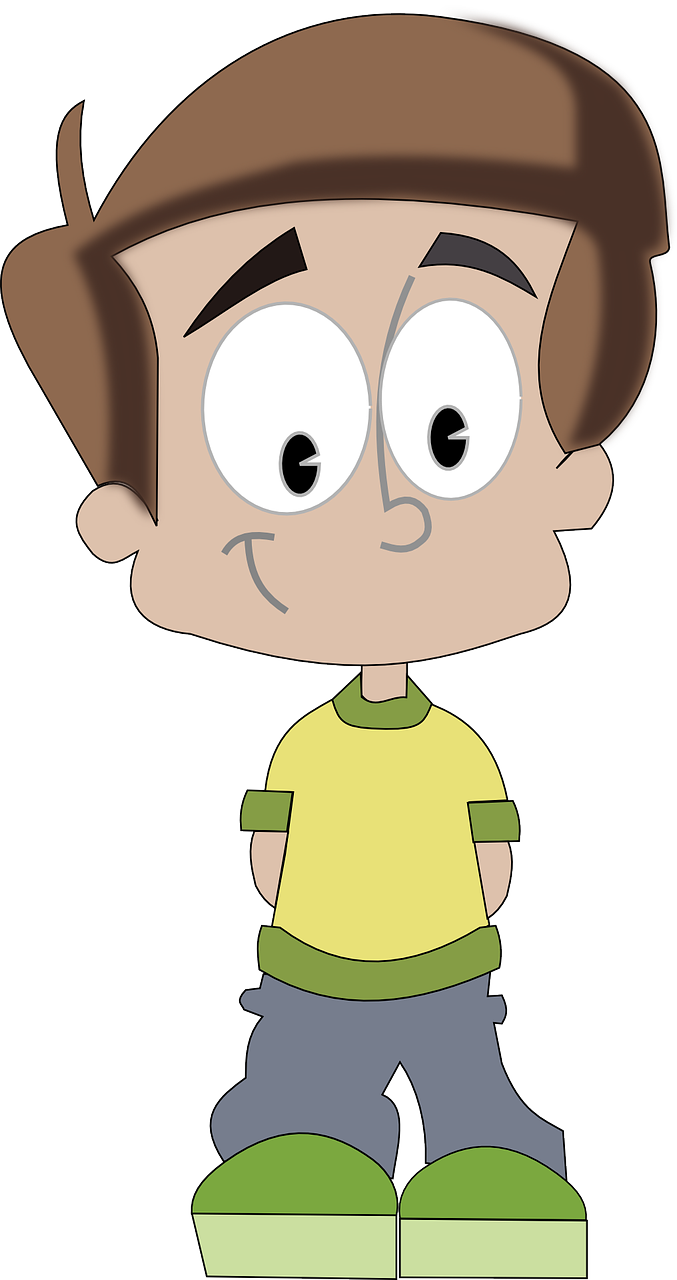
\includegraphics[width=1cm]{media/boy.png}};
    \coordinate (sun) at (7,12);
    \visible<2->{
      \fill [yellow] (sun) circle (1);
    }
    \visible<3->{
      \foreach \y in {10, 20, 30} 
      {
        \draw [very thick,yellow] ($(sun) + (-150+\y:1.1)$) -- ($(tree) + (80-2*\y:3)$) node [inner sep=0] (trays) {};
        \draw[very thick, green] (trays)-- ($(boy)+(0,0.6)$);
      }
    }
  \end{tikzpicture}

\end{frame}

\begin{frame}{How do we see things?}
  \begin{columns}
    \begin{column}{0.7\textwidth}
      \begin{itemize}
        \item
          Does the ``sight'' travel from our eyes to the object?\\
          \visible<2-> {\color{red}Euclid and other Greek philosophers believed so around 300 BC}
       \item
         \color{black}{or the ``light'' travels from the object to our eyes?}\\
         \visible<3-> {\color{red}Modern scientists still believe so.}
      \end{itemize}
    \end{column}
    \hspace{-2cm}
    \begin{column}{0.3\textwidth}
      \centering
        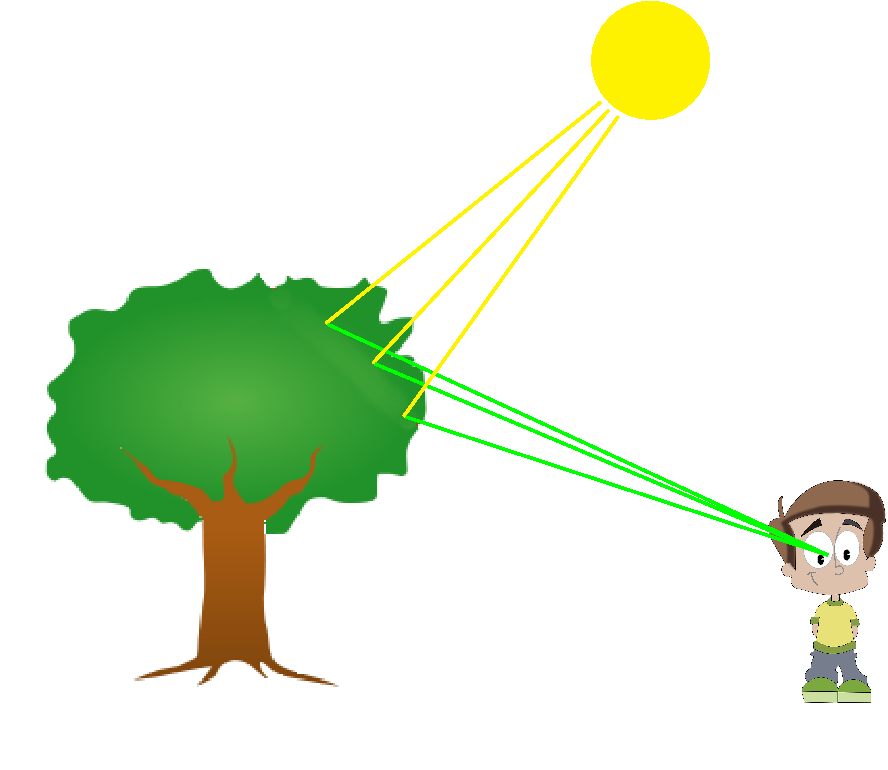
\includegraphics[width=1.4\textwidth]{media/suntreeboy.pdf}
    \end{column}
  \end{columns}
\end{frame}

\begin{frame}{What is light?}
  \begin{columns}
    \begin{column}{0.7\textwidth}
      \begin{itemize}
        \item Greek philosophers believed that sight was possible because of interaction of fire in eyes and in the sun.
        \item Euclid, a Greek philosopher, gave  us some particular insights about light.
      \end{itemize}
    \end{column}
    \begin{column}{0.3\textwidth}
      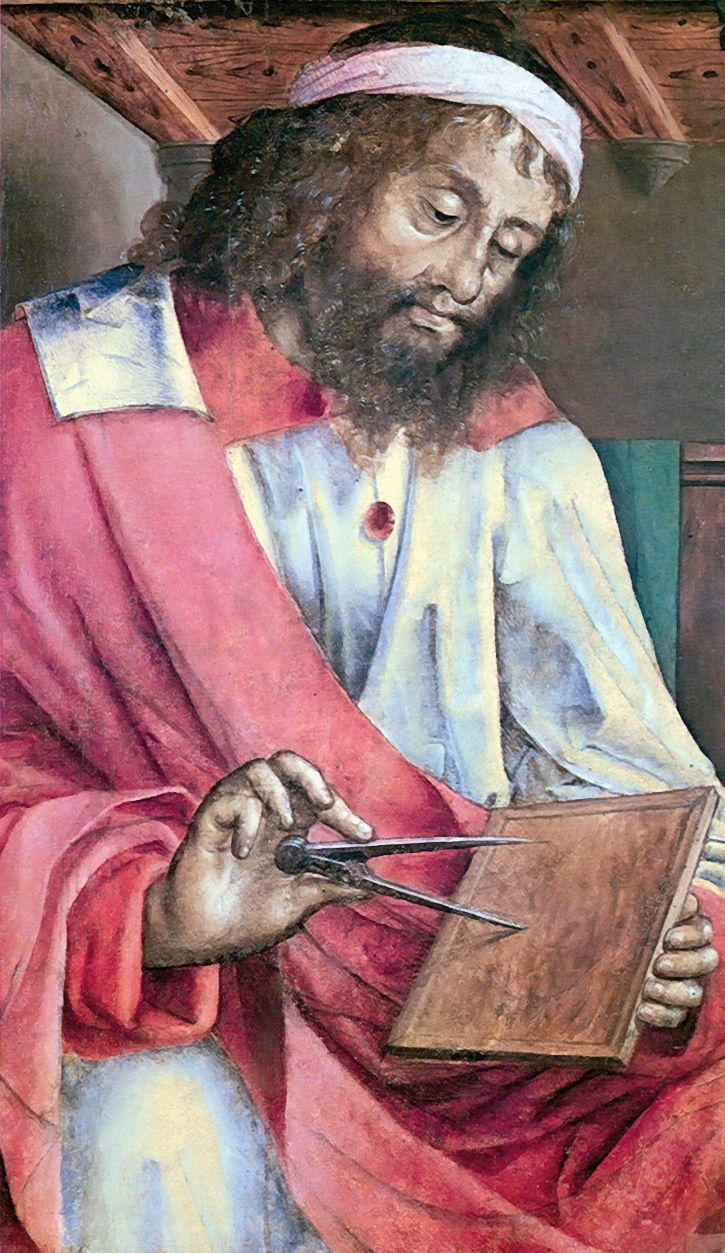
\includegraphics[width=\columnwidth]{media/Euklid.jpg}
    \end{column}
  \end{columns}
\end{frame}

\begin{frame}{Light travels in straight lines}
    \includemedia[label=euclid-straight-lines,
      width=\linewidth,height=0.6\linewidth, % 16:9
      activate=pageopen,
      addresource=media/euclid-straight-lines.mp4,
      flashvars={
        source=media/euclid-straight-lines.mp4
        &loop=false             % loop video
        &scaleMode=letterbox   % preserve aspect ratio while scaling the video
      }
    ]{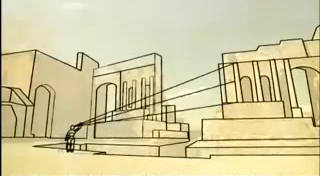
\includegraphics{media/euclid-straight-lines.png}}{VPlayer.swf}
    \footnotemark
  \footnotetext{BBC:Let there be Light (2006)}
\end{frame}

\begin{frame}{What is light?}
  Light is something that helps us see things. It travels in straight lines (mostly!!).
\end{frame}

\section{Making a pinhole camera}
\begin{frame}{Step 1}
  \begin{columns}
    \begin{column}{0.4\textwidth}
      Take a cup and scotch tape
    \end{column}
    \begin{column}{0.6\textwidth}
      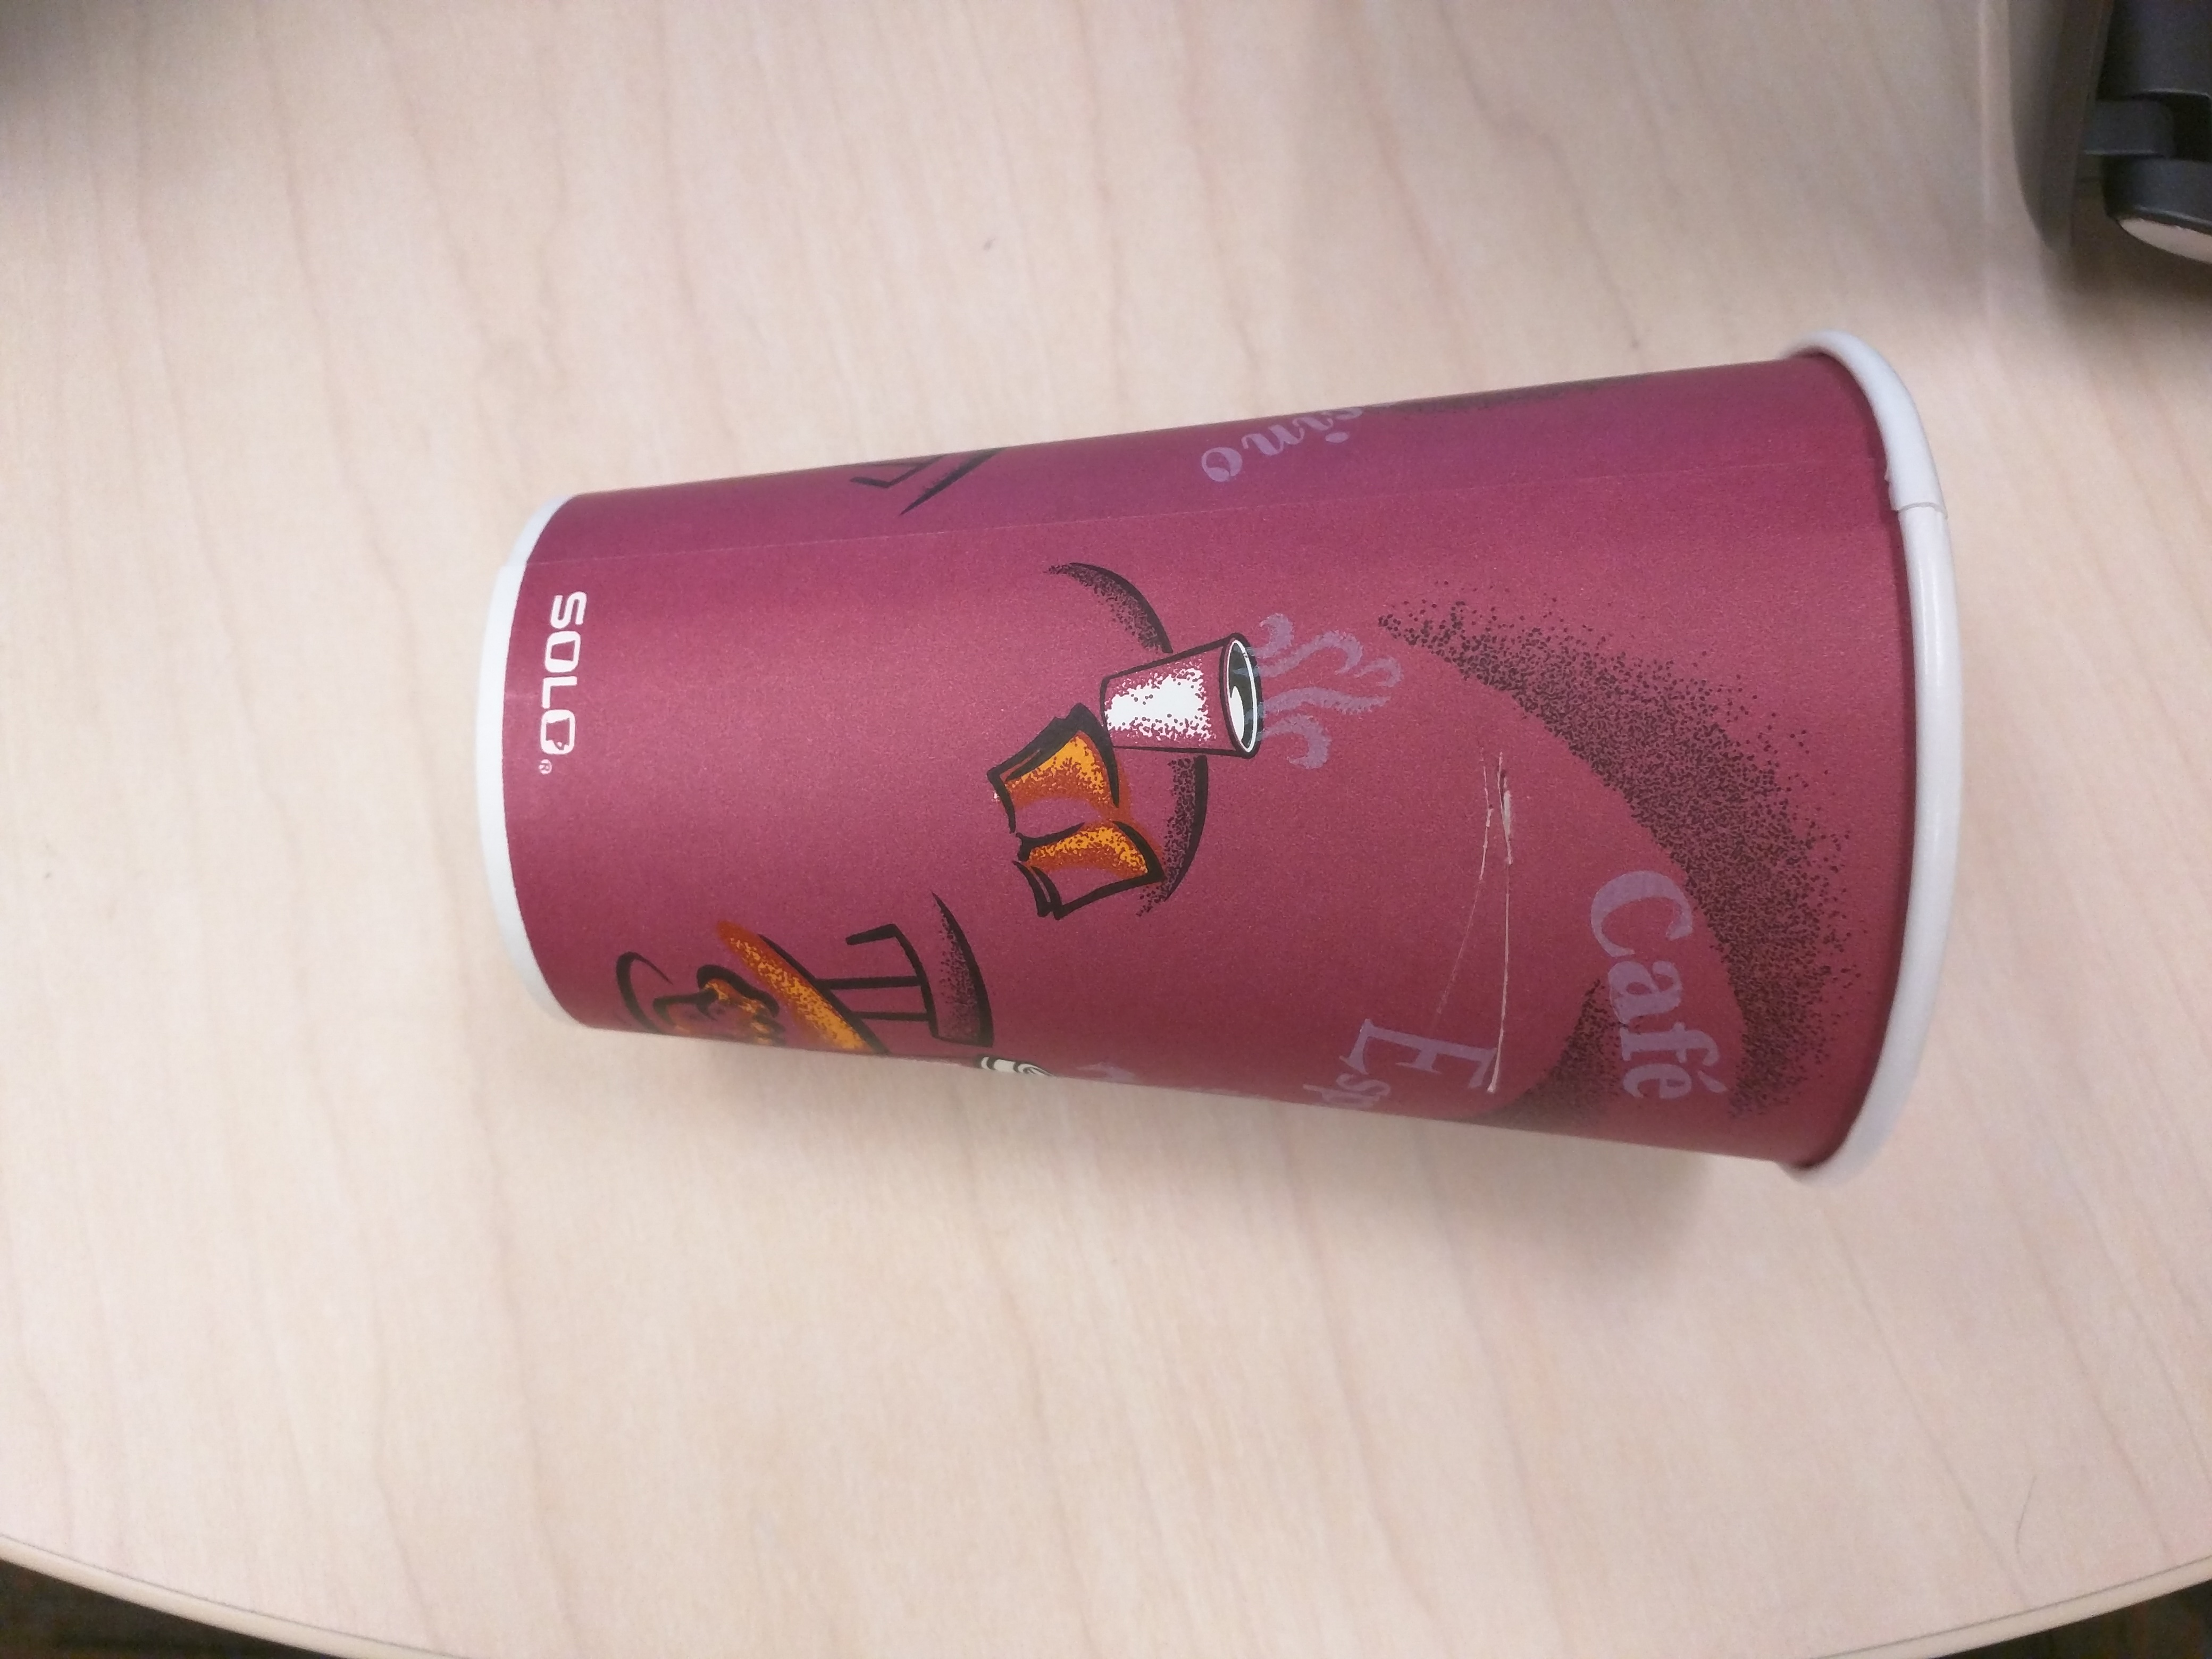
\includegraphics[width=\textwidth]{media/plain-cup.jpg}\\
      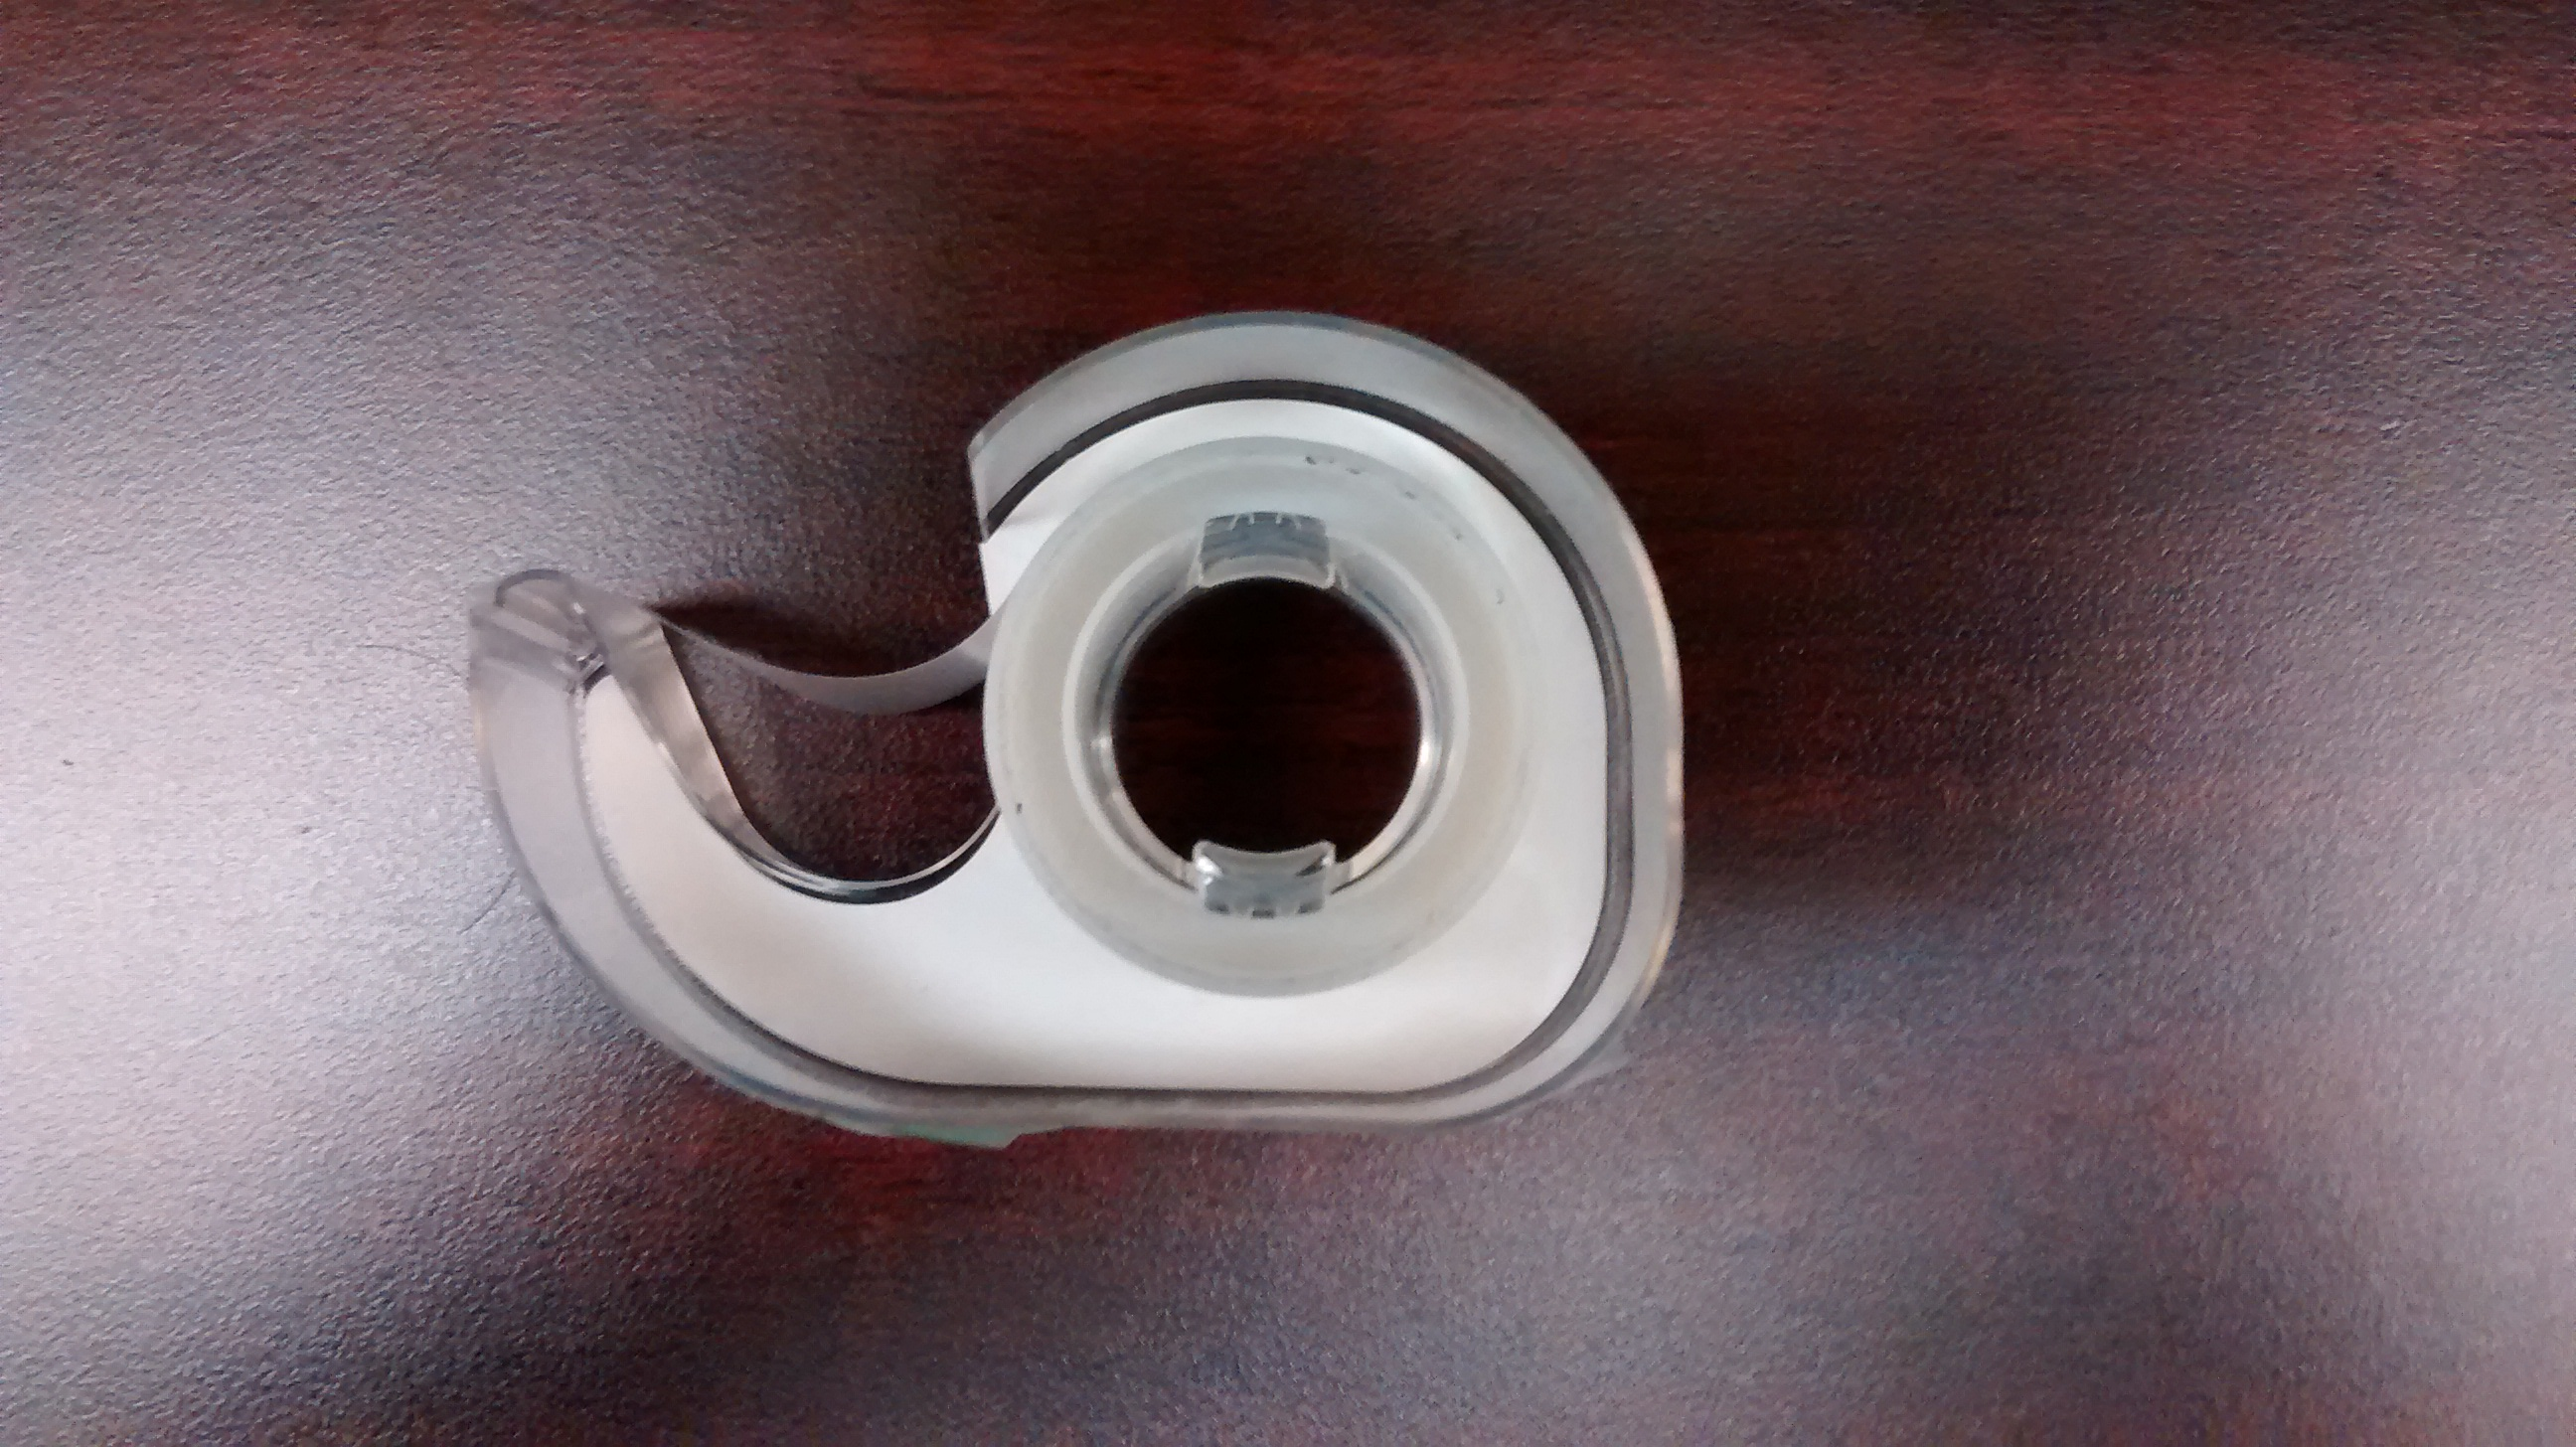
\includegraphics[width=\textwidth]{media/tape.jpg}
    \end{column}
  \end{columns}
\end{frame}

\begin{frame}{Step 2}
  \begin{columns}
    \begin{column}{0.6\textwidth}
      Cover the open end of cup using the scotch tape
    \end{column}
    \begin{column}{0.4\textwidth}
      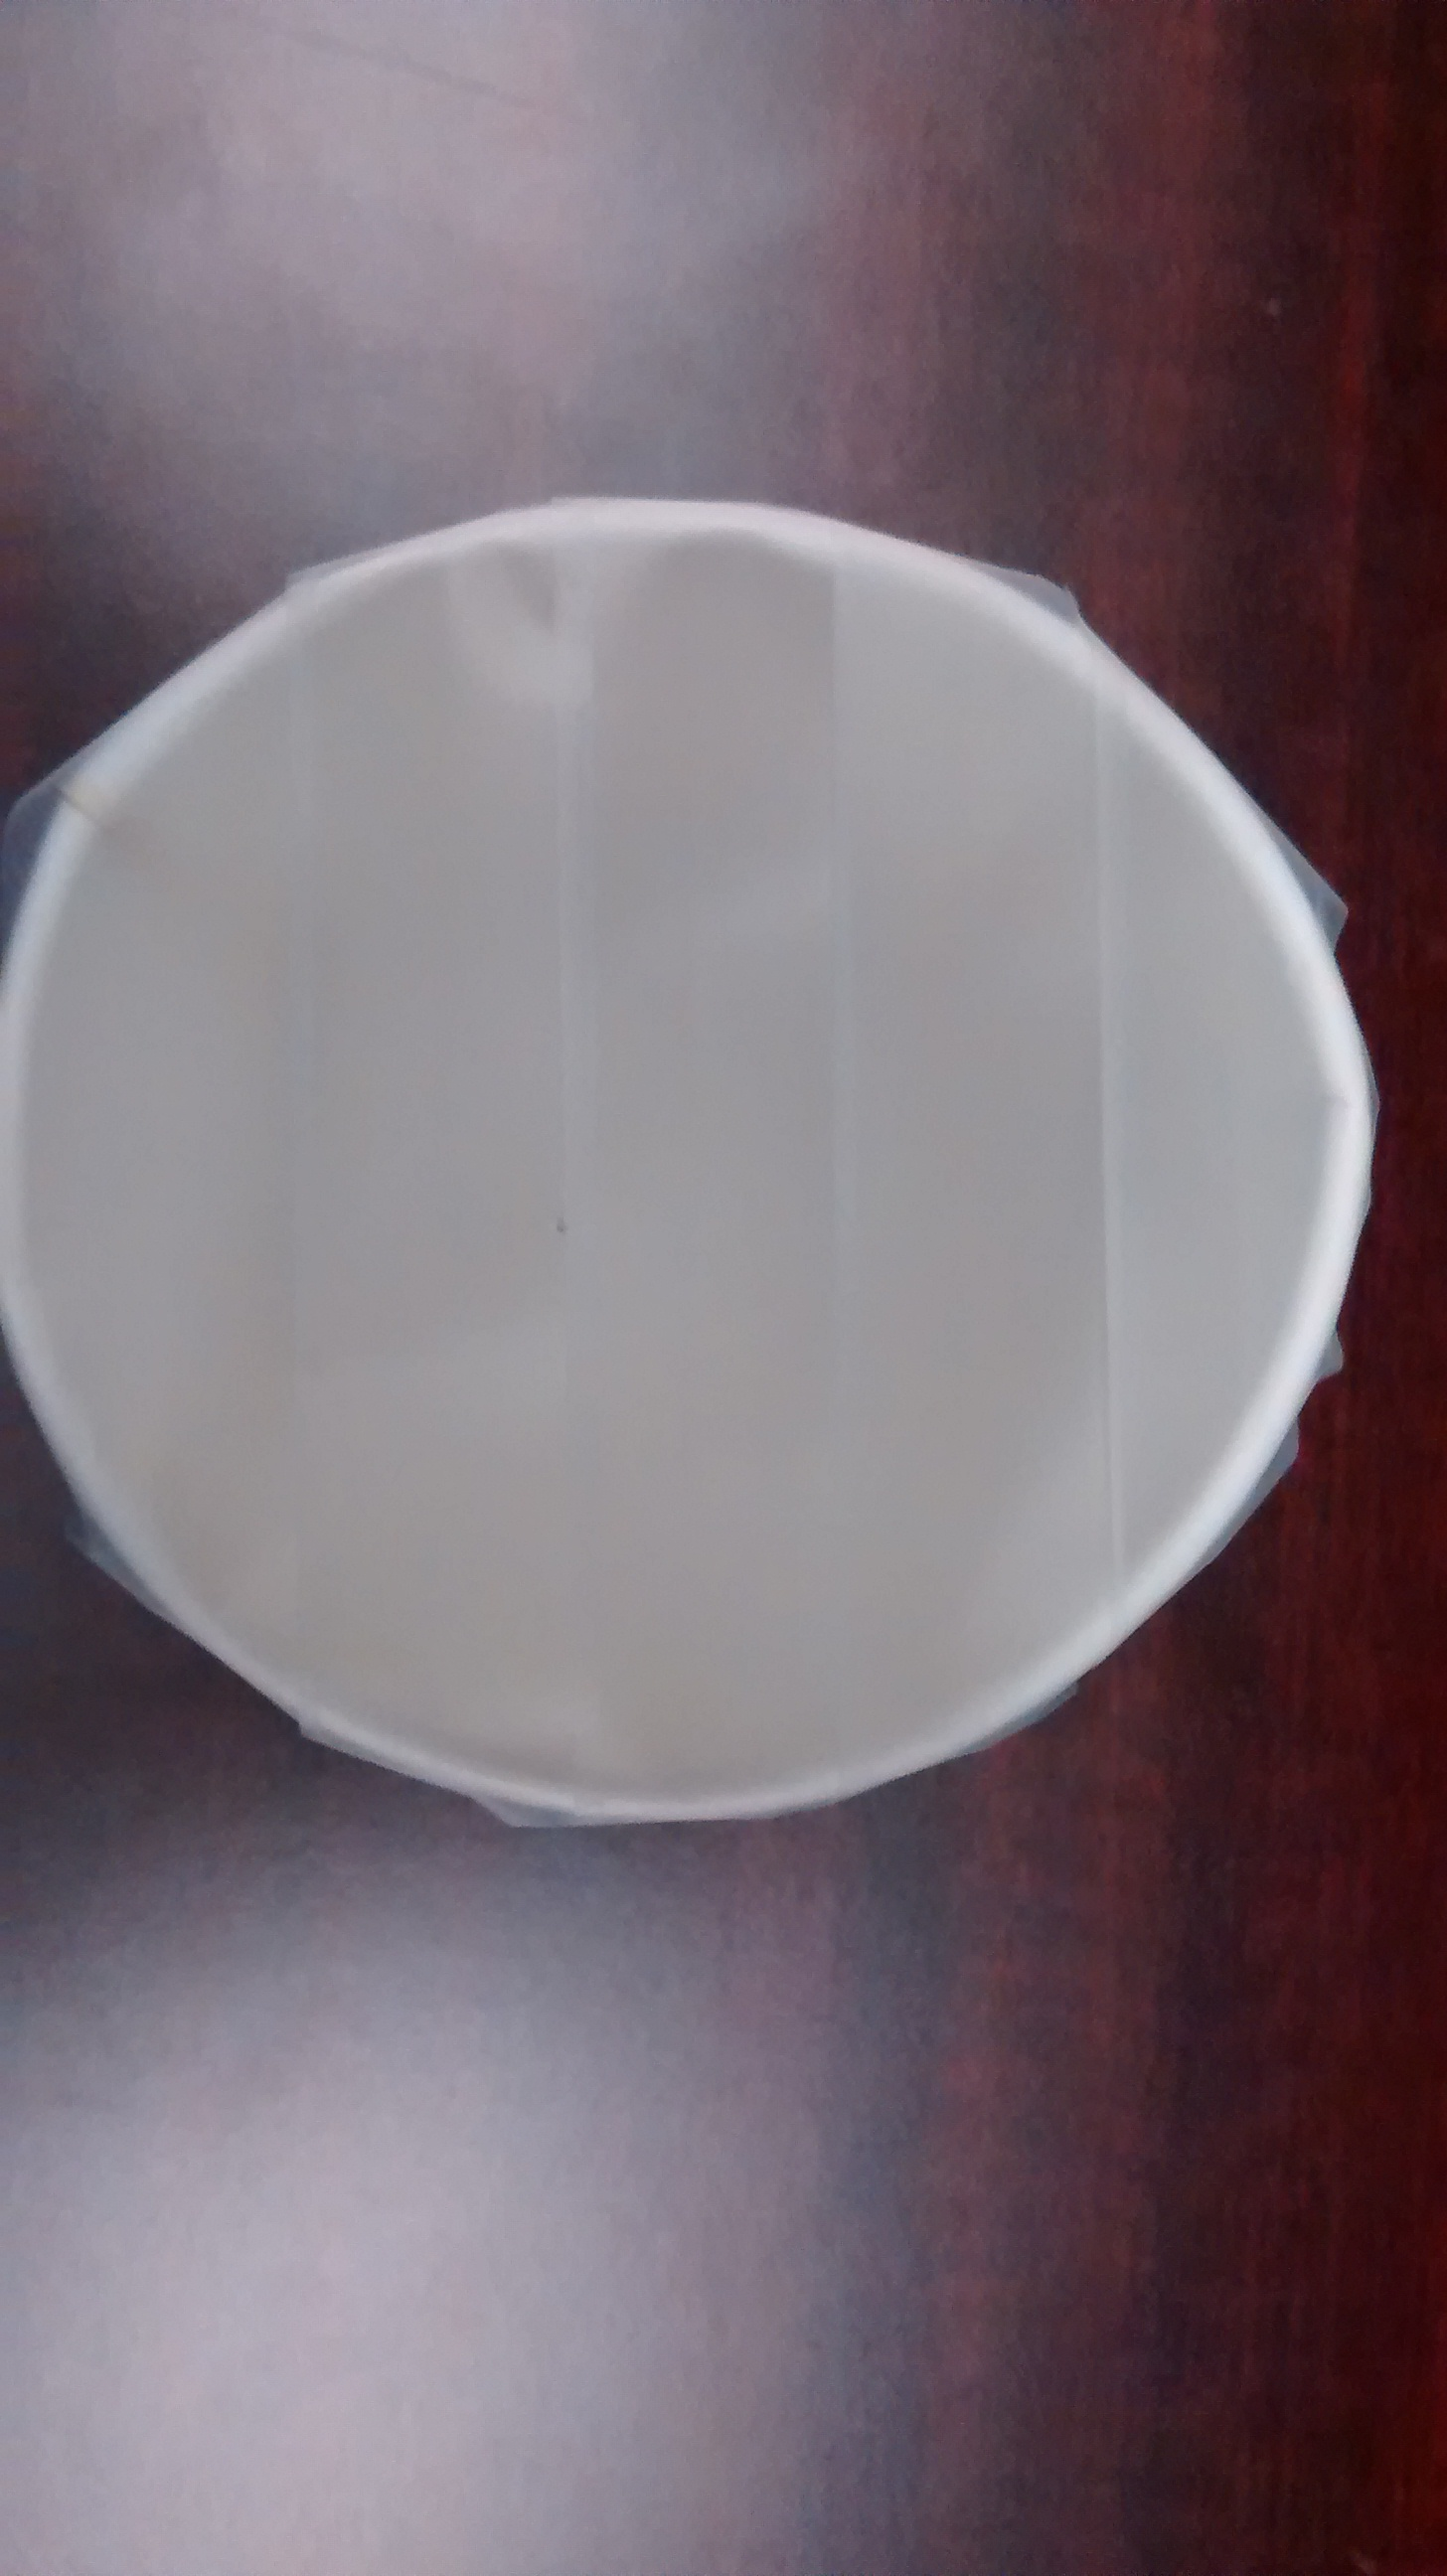
\includegraphics[width=\textwidth,trim=0 8in 0 4in,clip]{media/coveredlid2.jpg}\\
      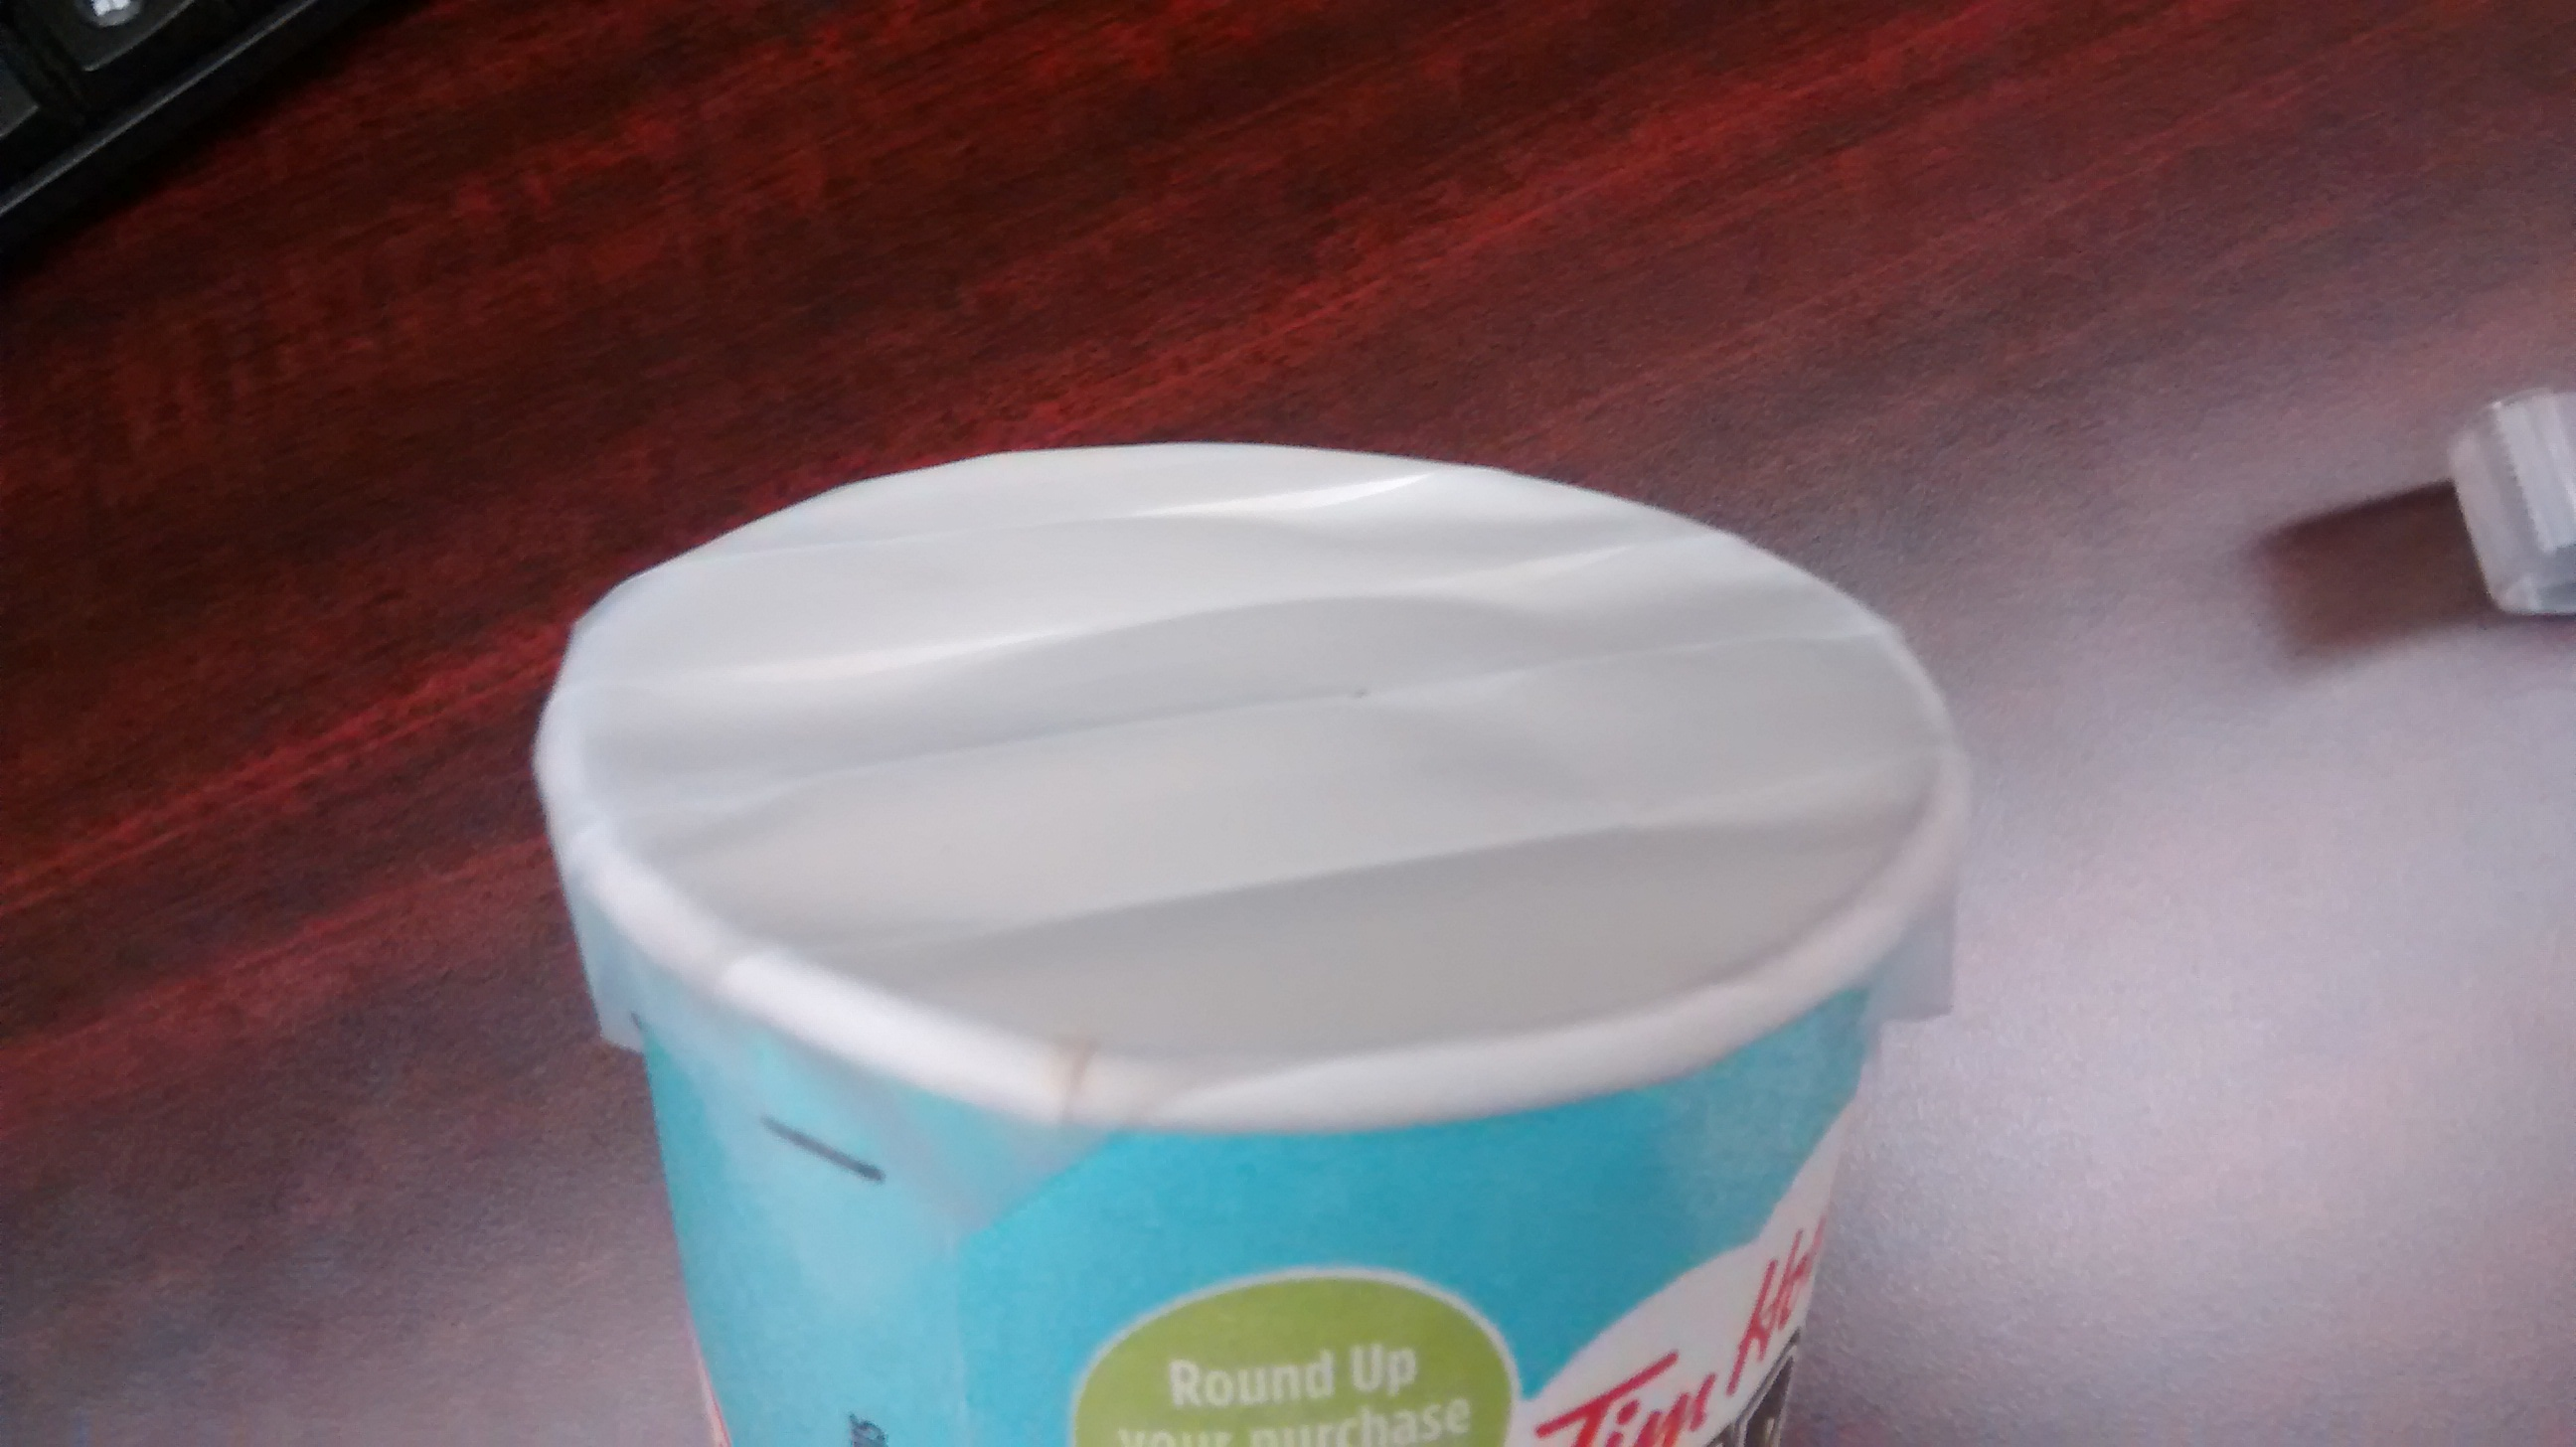
\includegraphics[width=\textwidth,trim=4in 0 4in 0,clip]{media/coveredlid1.jpg}
    \end{column}
  \end{columns}
\end{frame}

\begin{frame}{Step 3}
  \hl{TODO:Put a picture of cup without push pin}
  \begin{columns}
    \begin{column}{0.6\textwidth}
      Cut a circular piece of construction paper to reinforce the cup base.
    \end{column}
    \begin{column}{0.4\textwidth}
      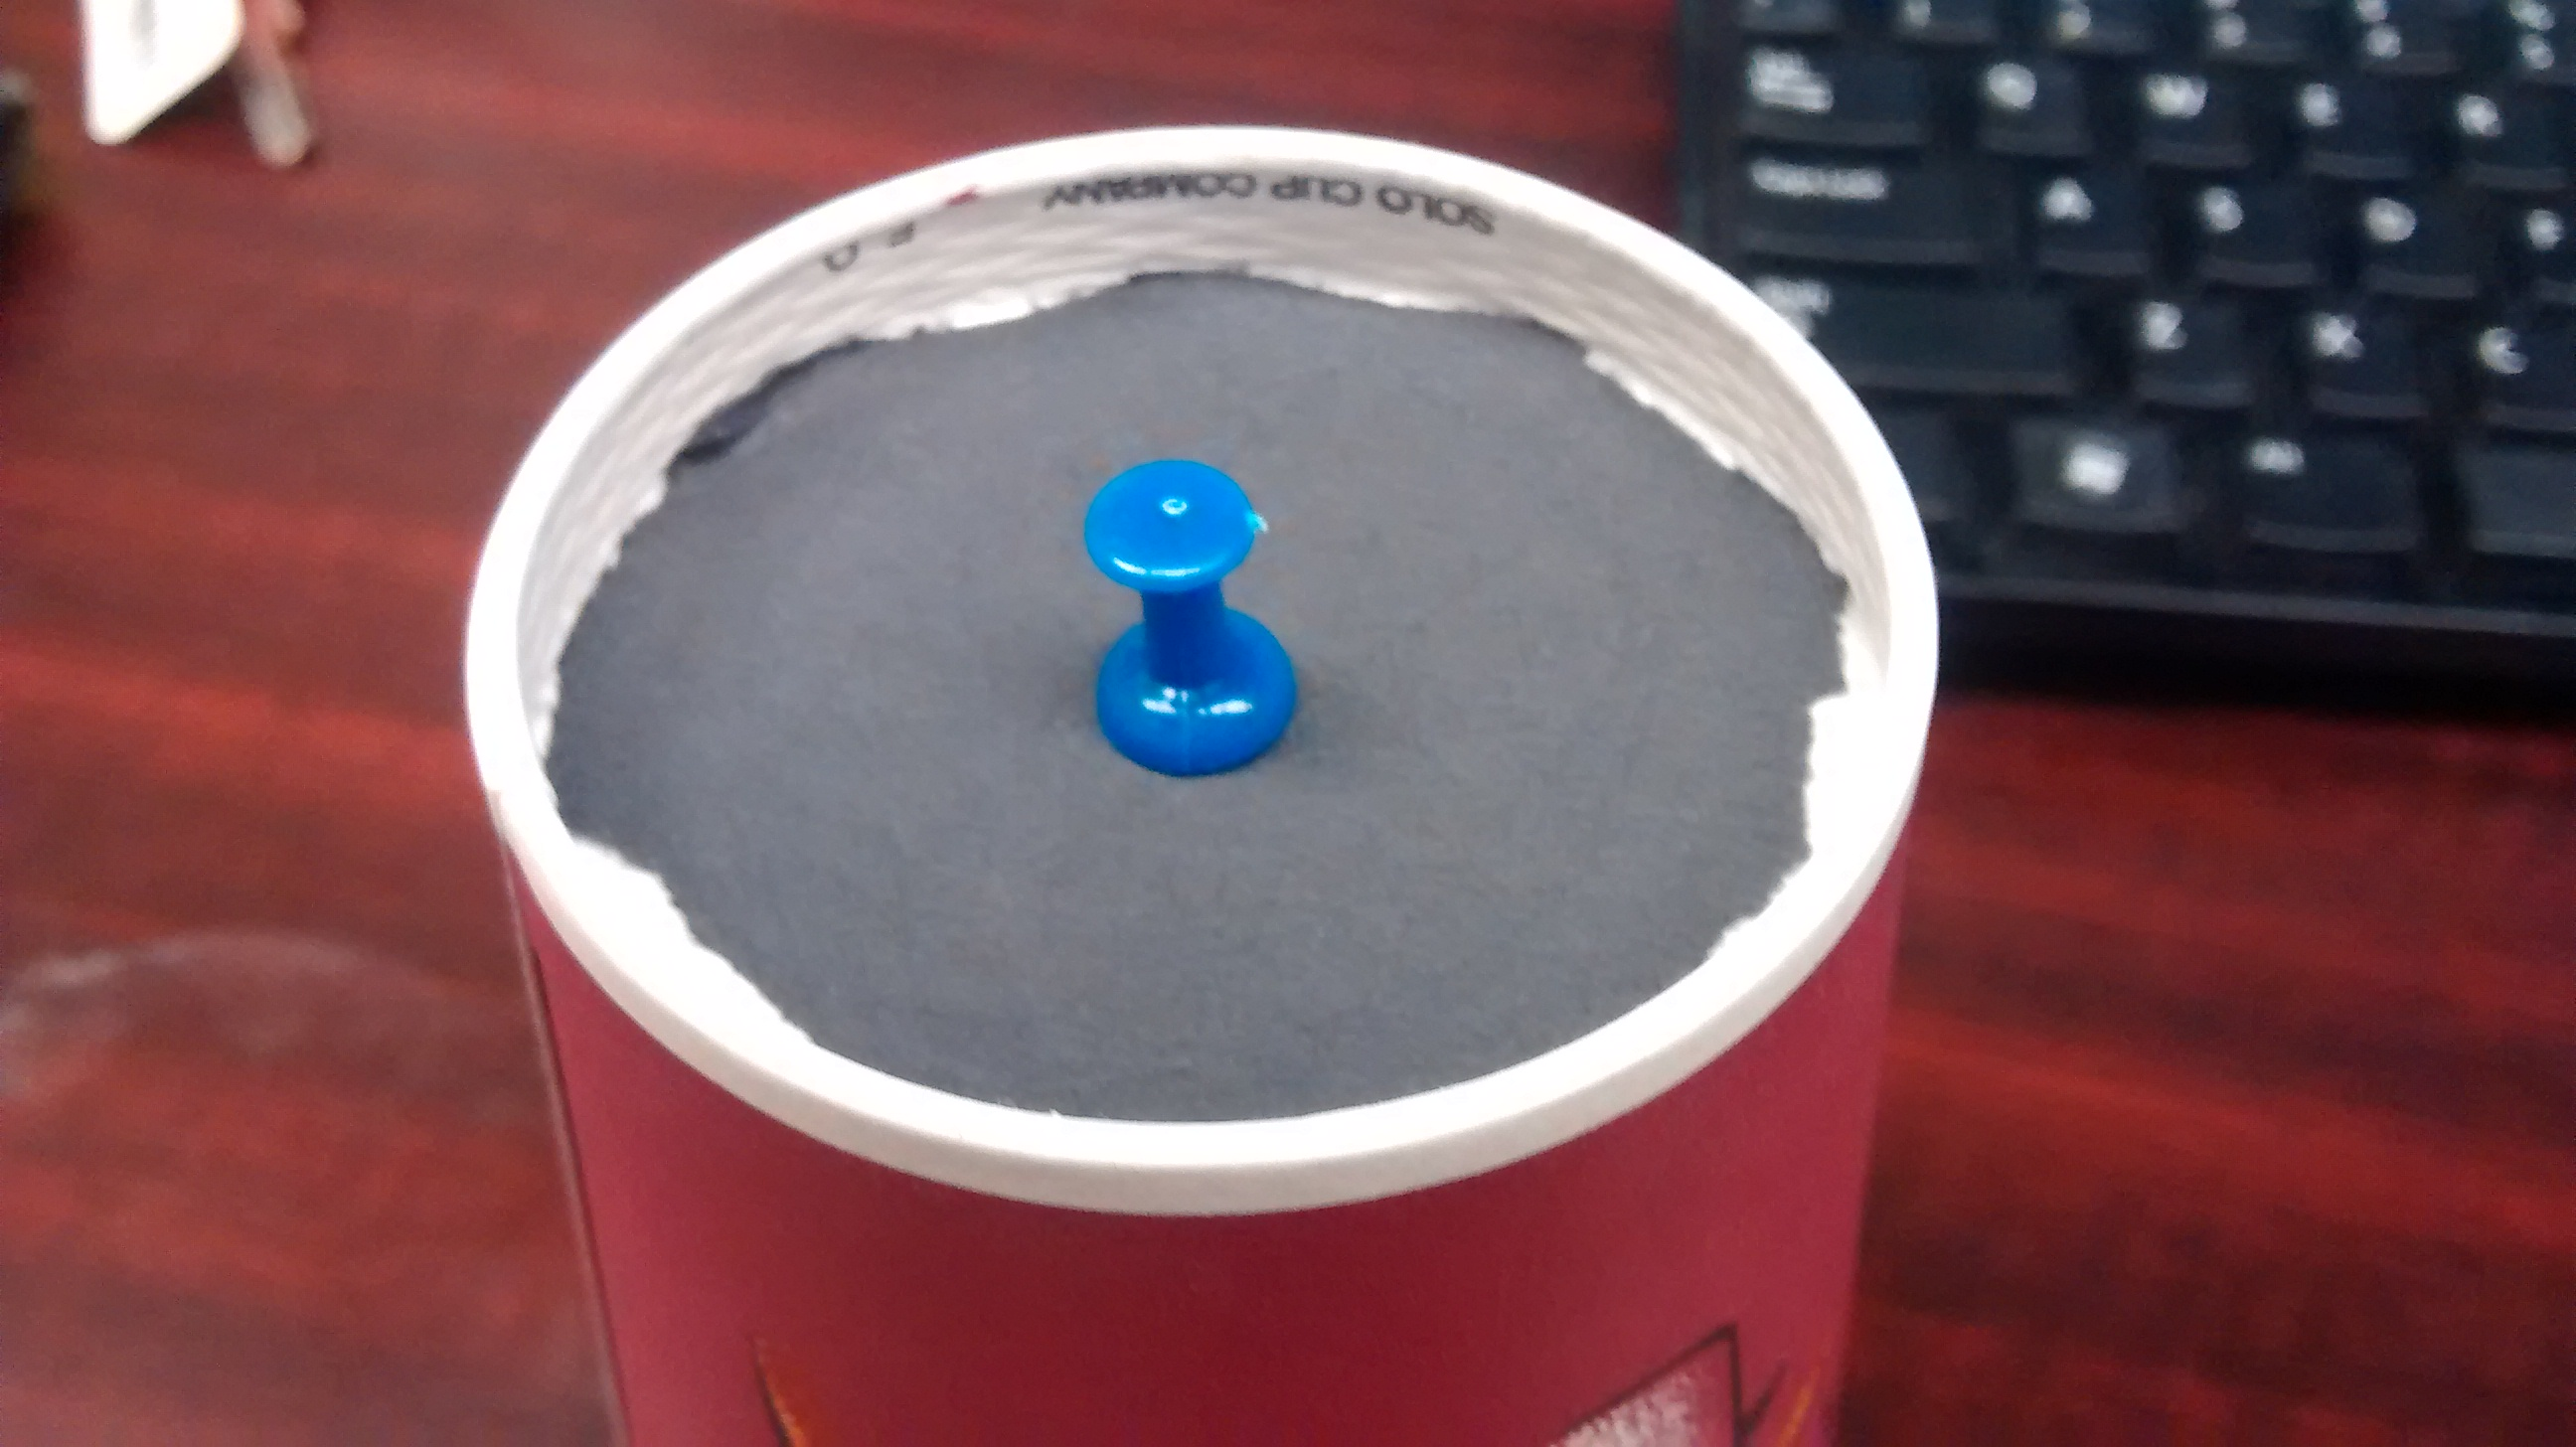
\includegraphics[width=\textwidth]{media/pushpin.jpg}
    \end{column}
  \end{columns}
  
\end{frame}

\begin{frame}{Step 4}
  \hl{TODO:Put a picture of cup without push pin but with a hole}
  \begin{columns}
    \begin{column}{0.6\textwidth}
      Pierce a pinhole through the closed end of the cup using a push pin
    \end{column}
    \begin{column}{0.4\textwidth}
      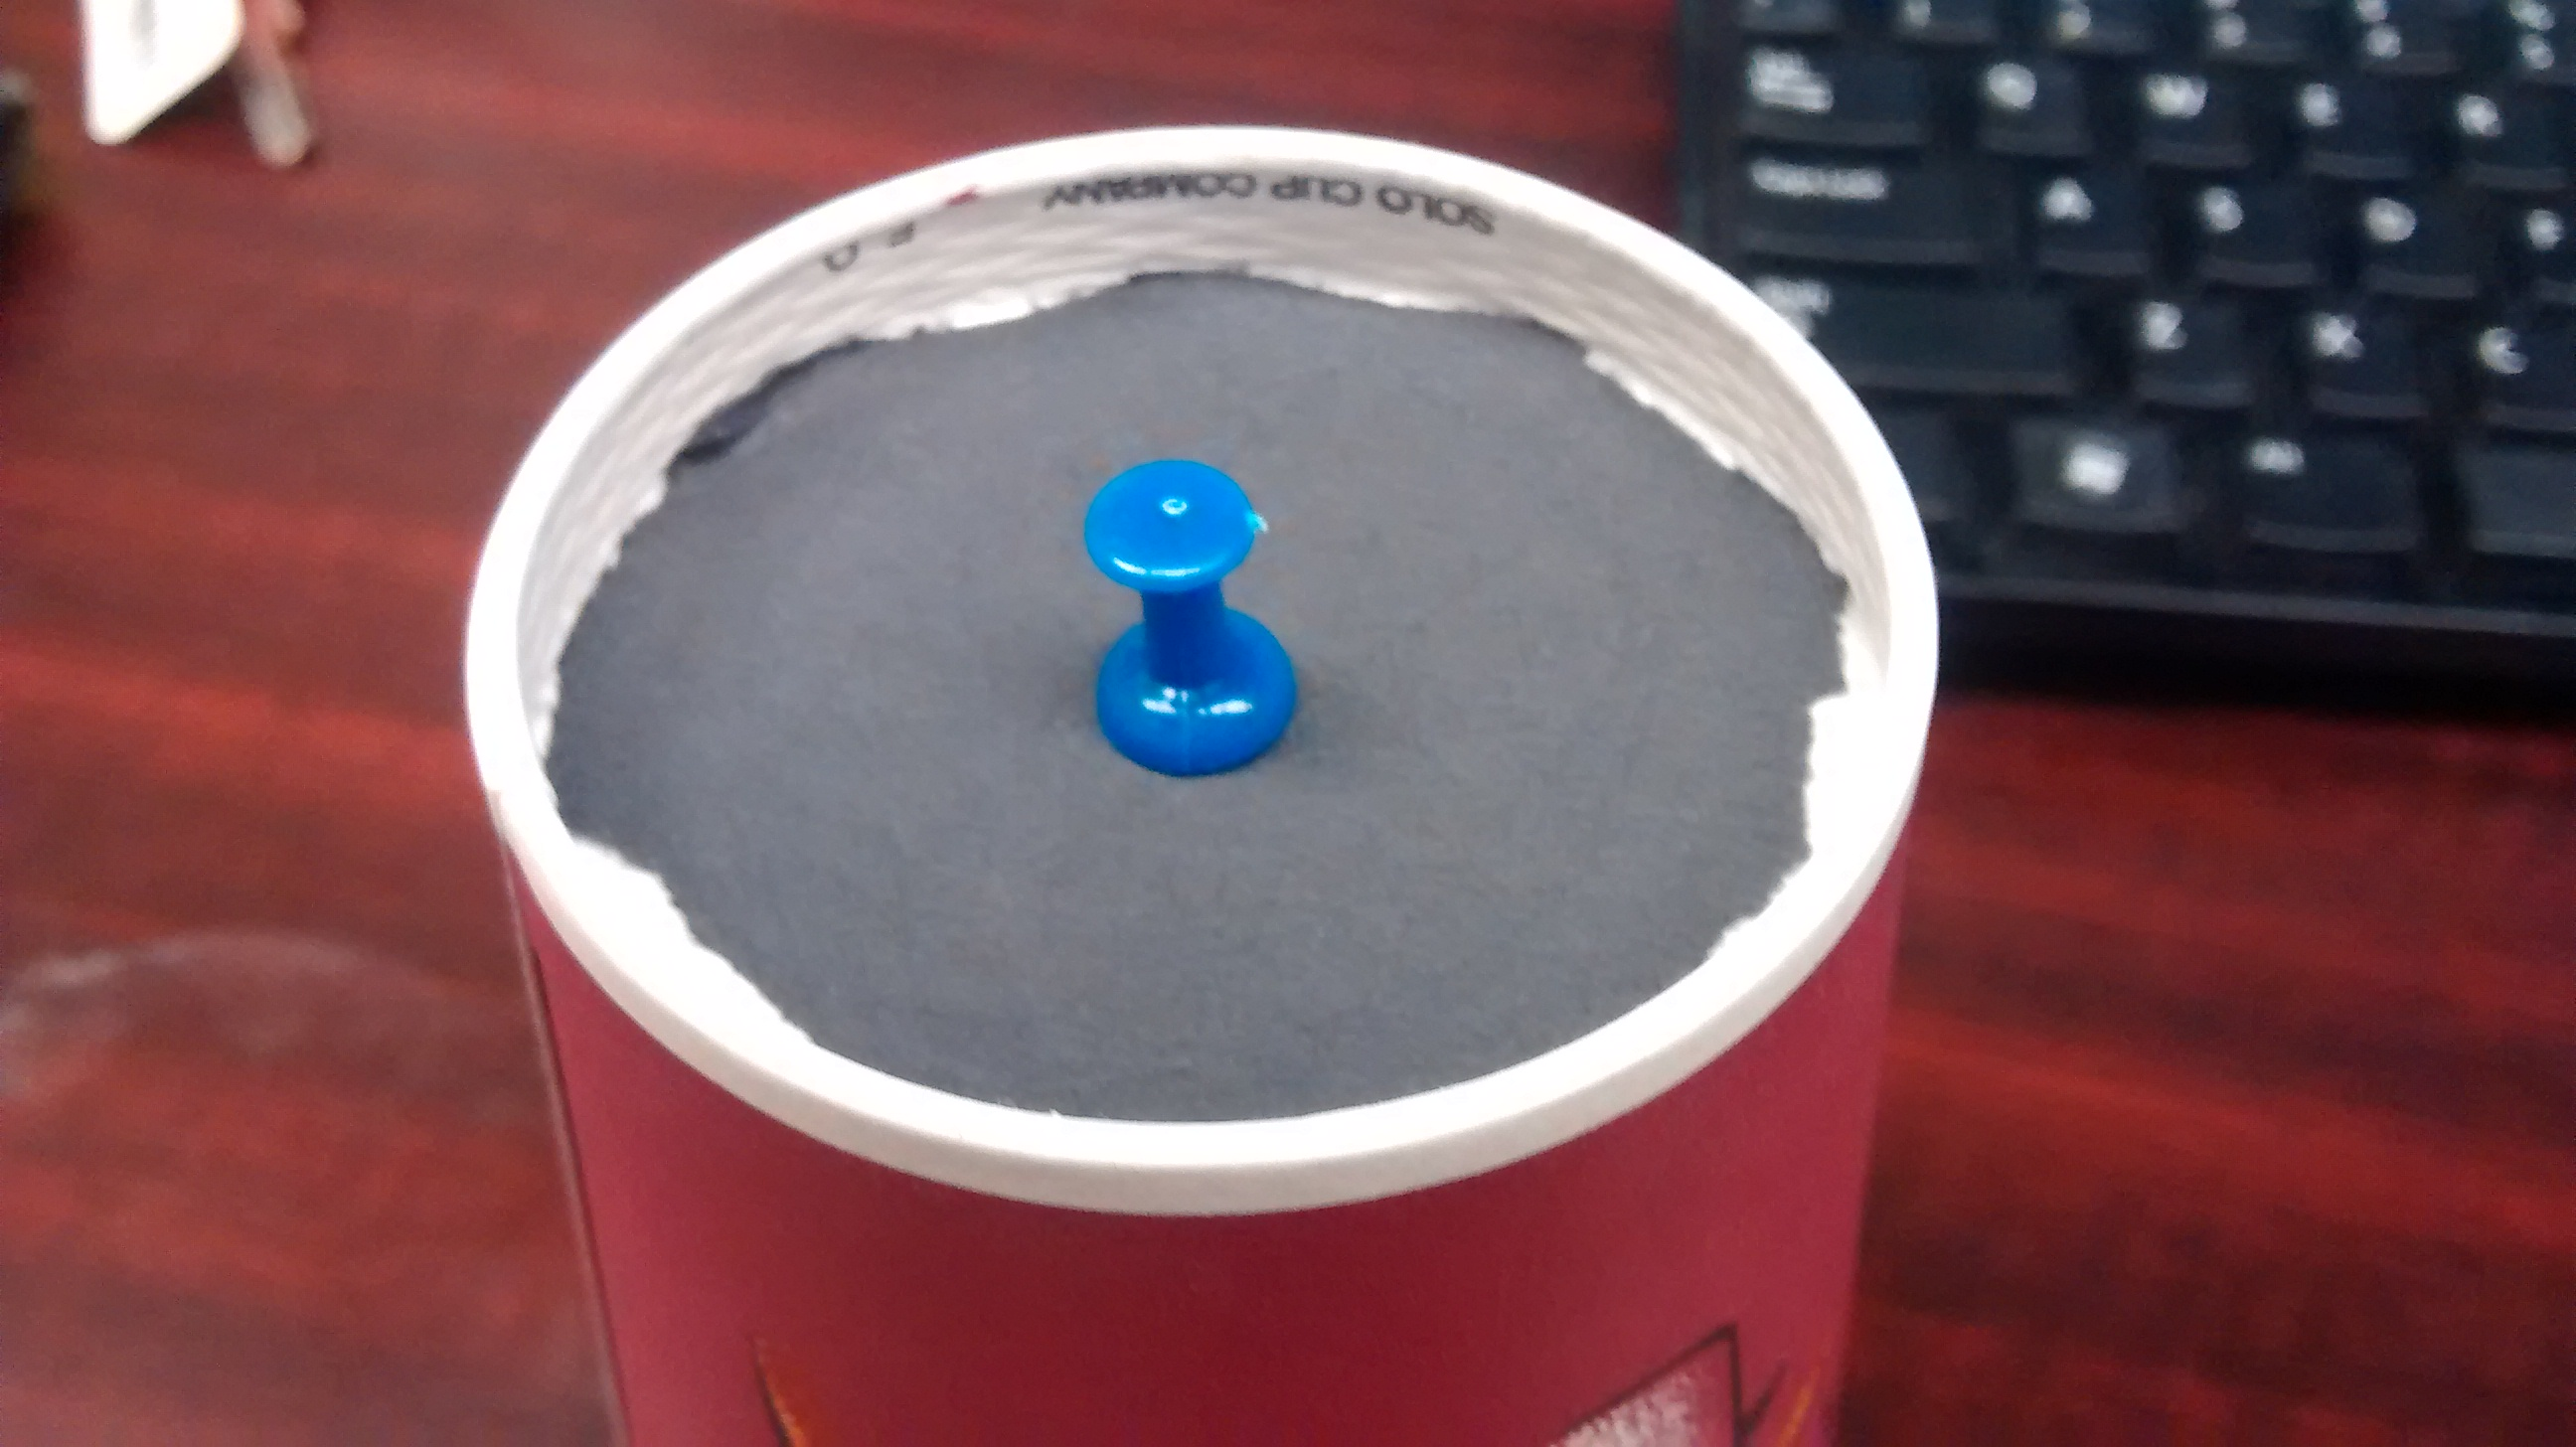
\includegraphics[width=\textwidth]{media/pushpin.jpg}
    \end{column}
  \end{columns}
\end{frame}

\begin{frame}{Using the pinhole camera}
  \hl{TODO:Show a picture of how to use the camera}
  \begin{itemize}
    \item
      Point the bottom of the cup towards the object and scotch tape towards you.\\
    \item
      Hold the cup around one foot away from your eyes.
  \end{itemize}
\end{frame}

\begin{frame}{Experiment time}
  We will turn on the bulb.
\end{frame}

\begin{frame}
  \addtooverlay<1->{%
    \draw[fill=black,opacity=1.00] 
    (current page.north east) rectangle (current page.south west);
    \node at (current page.center) {
\includegraphics[height=\textheight]{media/tree.png}};
  }
\end{frame}

\begin{frame}{Did you see an inverted image?}
  \begin{center}
    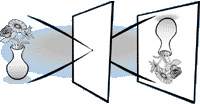
\includegraphics{media/upside_down_vase.png}
  \end{center}
\end{frame}

\section{How does it work}
\begin{frame}{Ray diagram}
  \begin{tikzpicture}[scale=0.8]
    \node [anchor=south west] (img) at (0,0) {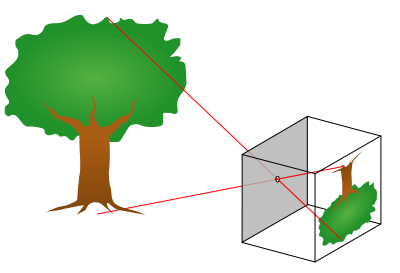
\includegraphics[width=0.8\textwidth]{media/pinhole.png}};
    \begin{scope}[x={(img.south east)},y={(img.north west)}]
      \fill [yellow] (0.75,1.2) node (sun) {} ellipse (0.06 and 0.08);
\coordinate (tree) at (0.2,0.7);
      \foreach \y in {10, 20, 30} 
      {
        \draw [very thick,yellow] ($(sun) + (-150+\y:.1)$) -- ($(tree) + (80-2*\y:.3)$) node [inner sep=0] (trays) {};
	}
    \end{scope}
  \end{tikzpicture}
\end{frame}

\begin{frame}{Camera Obscura: Camera in a room}
    \includemedia[label=camera-ina-room,
      width=\linewidth,height=0.6\linewidth, % 16:9
      activate=pageopen,
      addresource=media/camera_ina_room.mp4,
      flashvars={
        source=media/camera_ina_room.mp4
        &loop=false             % loop video
        &scaleMode=letterbox   % preserve aspect ratio while scaling the video
      }
    ]{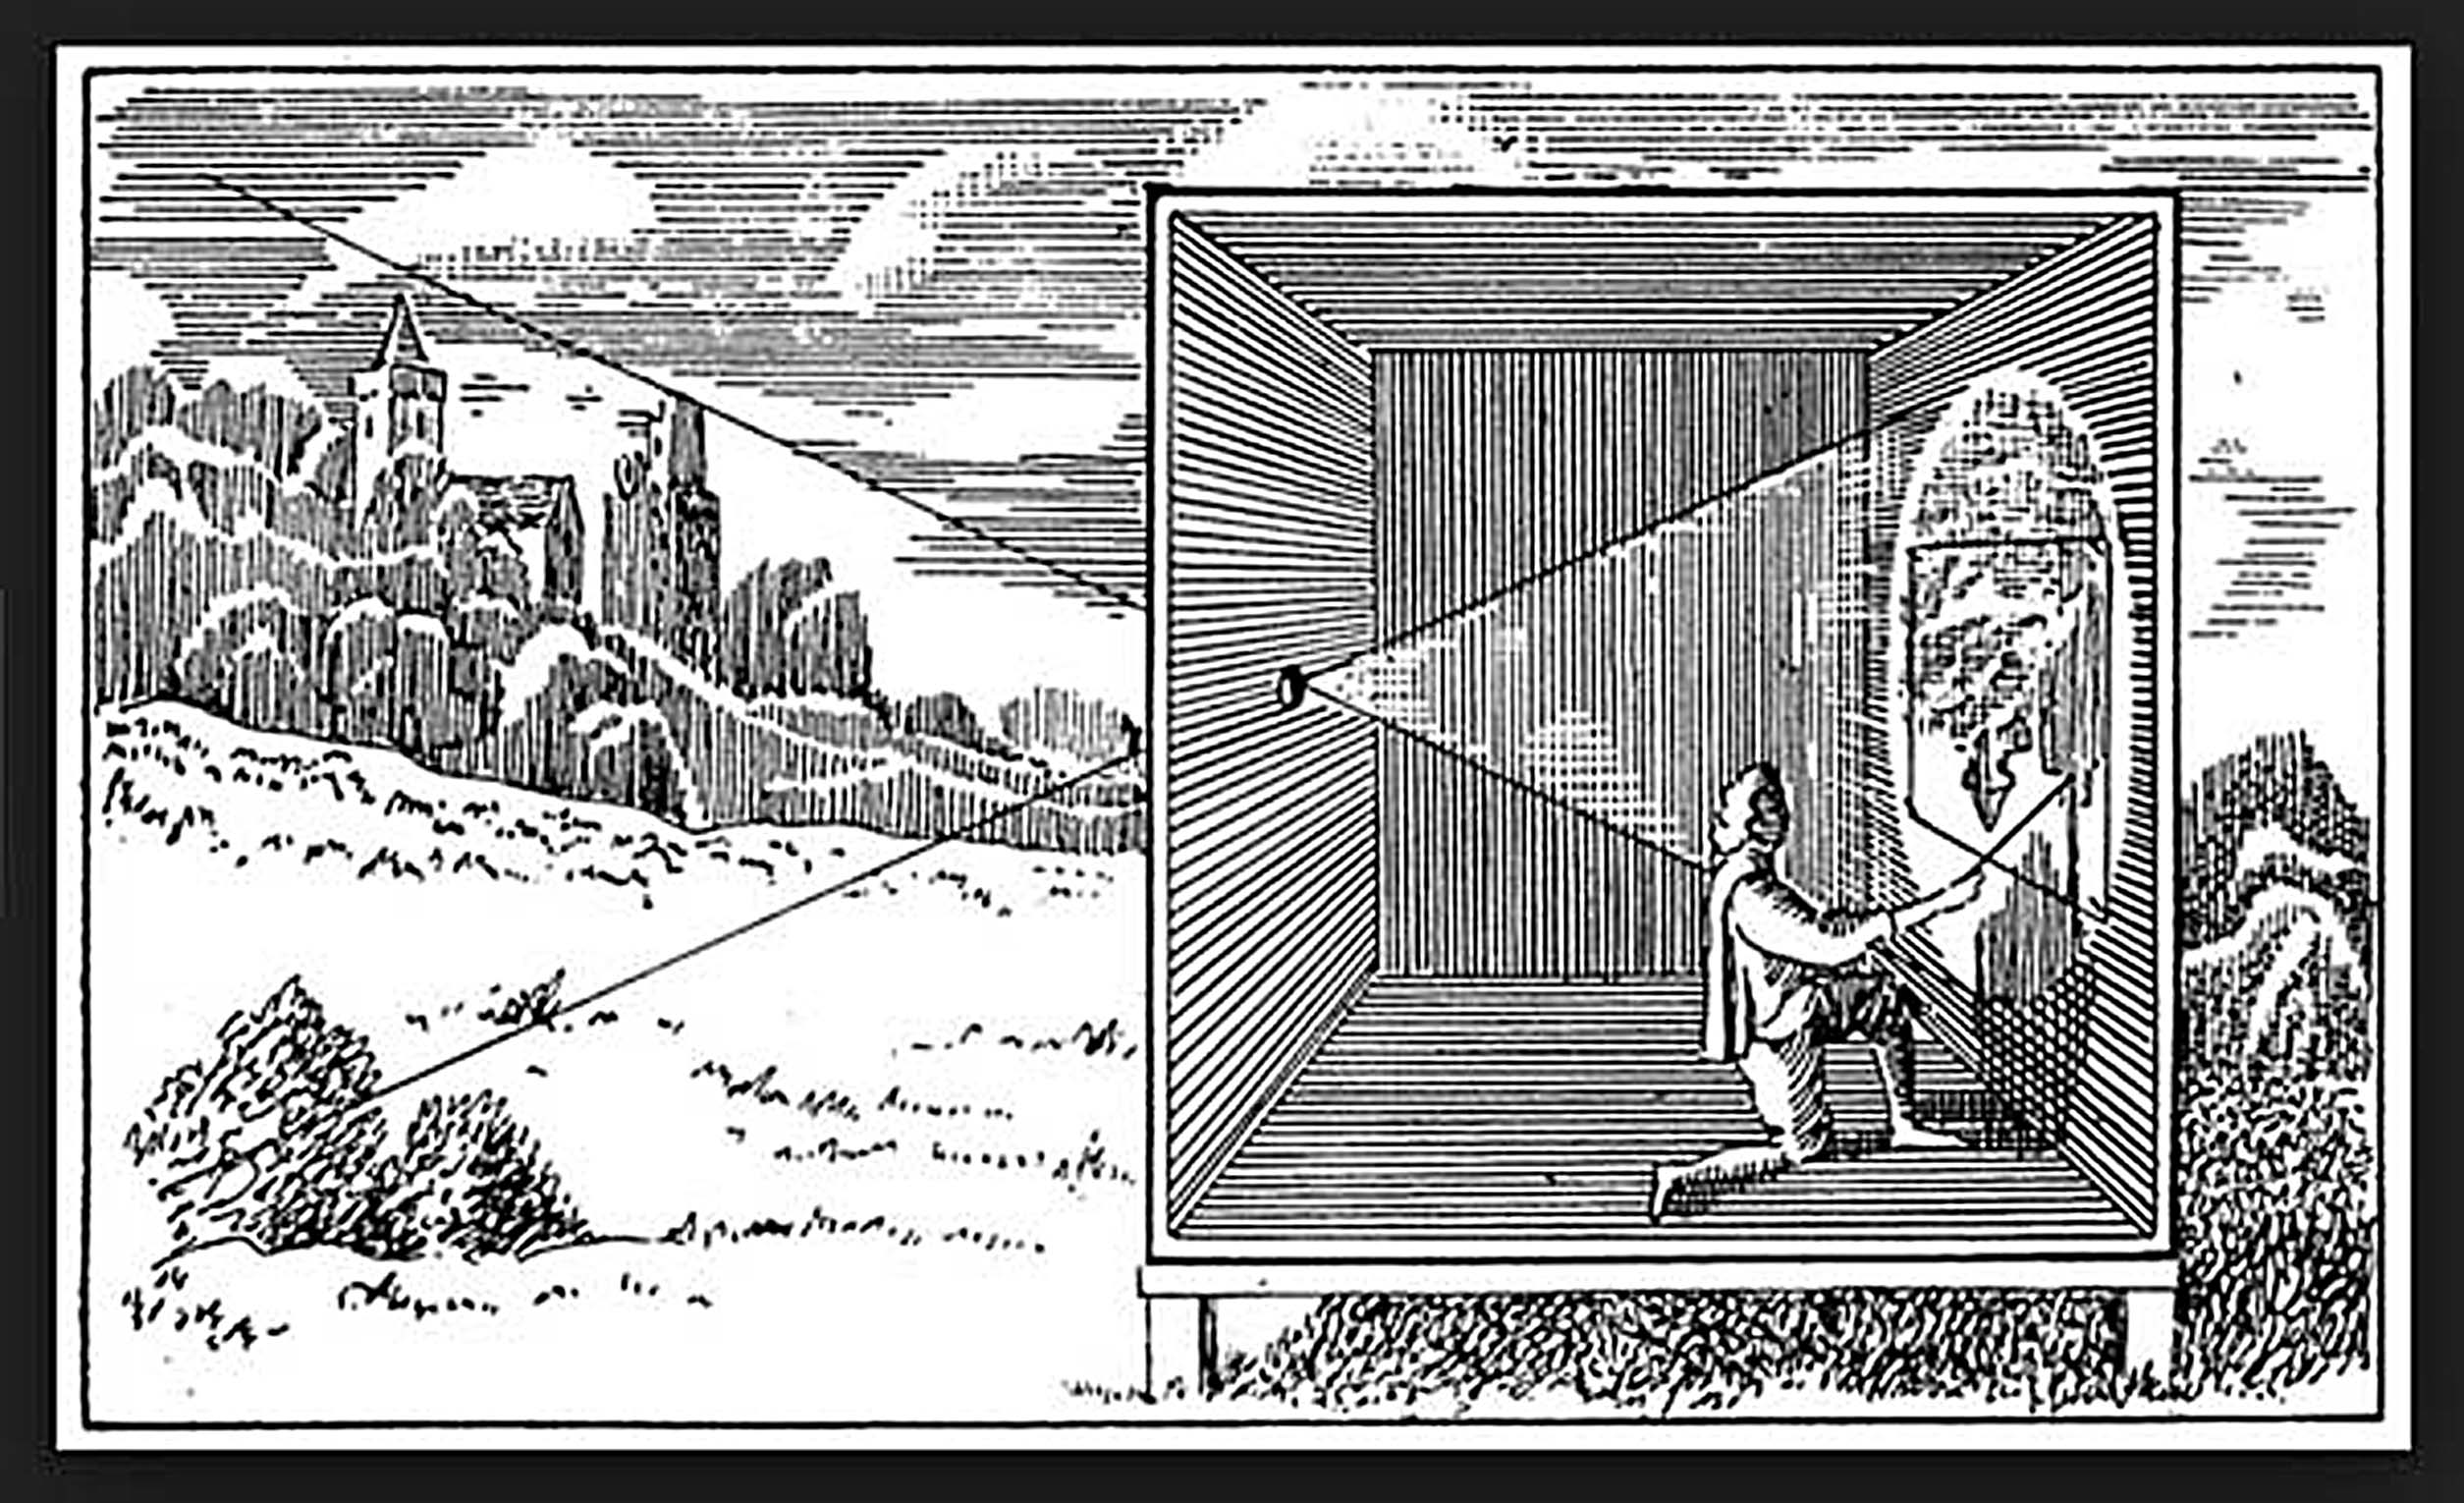
\includegraphics{media/camera_ina_room.jpg}}{VPlayer.swf}
\end{frame}

\begin{frame}{Camera Obscura: Camera in a room}
  \centering
  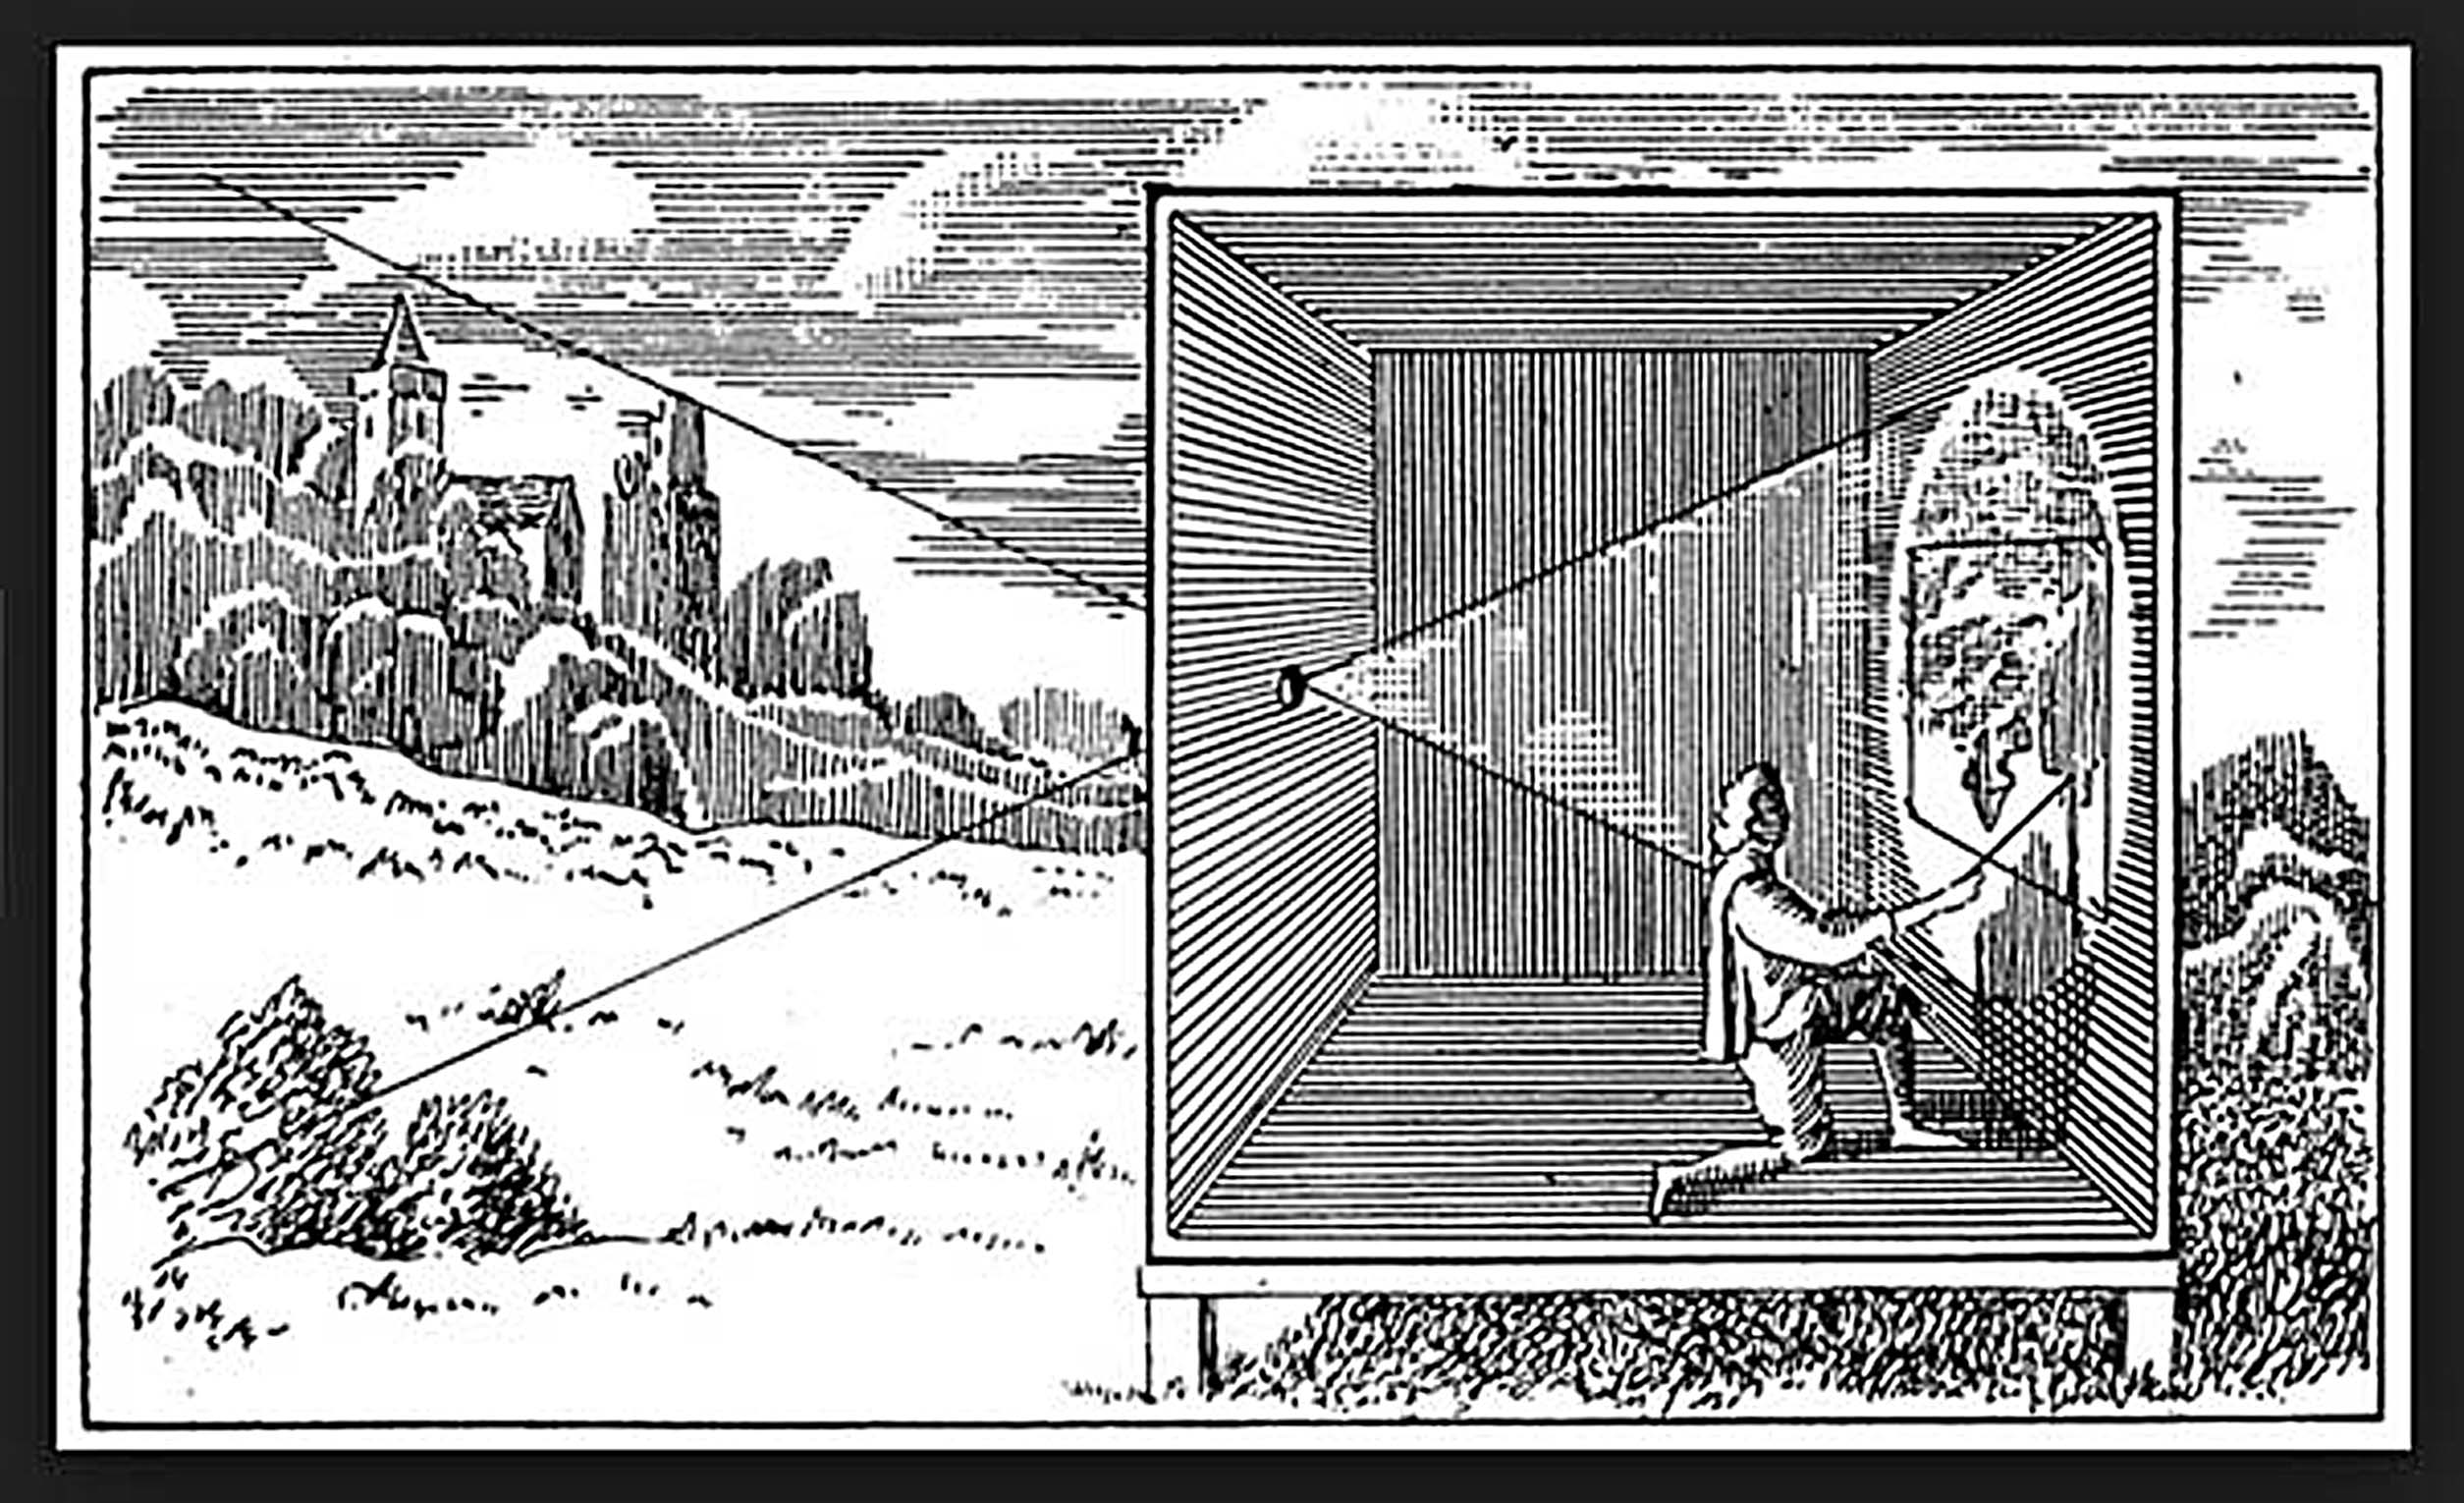
\includegraphics[width=\textwidth]{media/camera_ina_room.jpg}
\end{frame}

\section{Effect of distance}
\begin{frame}{Guess what happens}
  ... if you change the distance of the pinhole from the object?
\end{frame}

\begin{frame}[fragile]{Effect of distance}
  
             \newcommand{\textonecolor}[1]{\ifnum2<#1black\else black!50\fi}
  \only<2>{\renewcommand{\textonecolor}[1]{\ifnum3<##1black\else black!50\fi}}
  \only<4>{\renewcommand{\textonecolor}[1]{\ifnum4<##1black\else black!50\fi}}

             \newcommand{\nodeonecolor}[1]{\if3#1red!20\else none\fi}
  \only<2>{\renewcommand{\nodeonecolor}[1]{\if4##1red!20\else none\fi}}
  \only<4>{\renewcommand{\nodeonecolor}[1]{\if5##1red!20\else none\fi}}
  \begin{center}
    \begin{tikzpicture}[]

      \def \n {6}
      \def \radius {3}
      \def \margin {15} % margin in angles, depends on the radius

      \foreach \s/\t in {1/Purpose,2/Research,3/Hypothesis,4/Experiment,5/Analysis,6/Conclusion}
      {
        \node[fill=\nodeonecolor{\s},text=\textonecolor{\s},circle,minimum width=3] at ({360/\n * (\s - 1)}:\radius) {\t};
        \draw[->, >=latex] ({360/\n * (\s - 1)+\margin}:\radius) 
        arc ({360/\n * (\s - 1)+\margin}:{360/\n * (\s)-\margin}:\radius);
      }
    \end{tikzpicture}
    \addtooverlay<.(3)>{%
      \draw[fill=black,opacity=1.00] 
      (current page.north east) rectangle (current page.south west);
      \node at (current page.center) {
\includegraphics[height=\textheight]{media/tree.png}};
    }
  \end{center}

\end{frame}

\begin{frame}{Guess what happens}
  ... if you change the distance of the pinhole from the object?\\
  \pause
  {\color{red} Does it become bigger?}
\end{frame}

\begin{frame}{Relating distance with image size?}
  Can you find the distance of the object given the size of object.
\end{frame}

\begin{frame}{Similar triangles}
  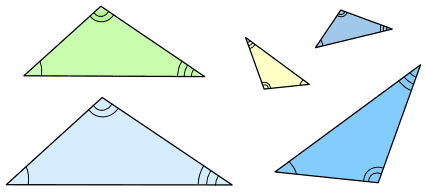
\includegraphics[width=\textwidth]{media/tri-similar1.png}
\end{frame}

\begin{frame}{Similar triangles}
  \begin{columns}
    \begin{column}{0.5\textwidth}
      \begin{tikzpicture}
        \def\la{A}
        \def\lb{B}
        \def\lc{C}
        \def\triangle{
        (0,0) node[anchor=north east] {\la} -- (1,2) node[anchor=south east] {\lb}-- (2,1) node [anchor=north west] {\lc} -- cycle;}
        \def\triangleanglearcs{
          \begin{scope}
            \clip \triangle;
            \draw [anglearcs] (0,0) circle (0.2);
            \draw [anglearcs] (1,2) circle (0.2);
            \draw [anglearcs] (1,2) circle (0.24);
            \draw [anglearcs] (2,1) circle (0.20);
            \draw [anglearcs] (2,1) circle (0.24);
            \draw [anglearcs] (2,1) circle (0.28);
          \end{scope}
        }
        \begin{scope}[anglearcs/.style={blue}]
          \draw [blue] \triangle;
          \triangleanglearcs
        \end{scope}
        \def\la{P}
        \def\lb{Q}
        \def\lc{R}
        \begin{scope}[rotate=30,shift={(3,-2)},scale=1.5,anglearcs/.style={red}]
          \draw [red] \triangle;
          \triangleanglearcs
        \end{scope}
      \end{tikzpicture}
    \end{column}
    \begin{column}{0.5\textwidth}   
      \begin{align*}
        &\angle ABC = \angle PQR \\
        &\land \angle BCA = \angle QRP \\
        &\iff \bigtriangleup ABC \sim \bigtriangleup PQR \\
        &\iff \frac{AB}{PQ} = \frac{BC}{QR} = \frac{CA}{RP}
      \end{align*}
    \end{column}
  \end{columns}
\end{frame}

\begin{frame}{Geometry of pinhole camera}
  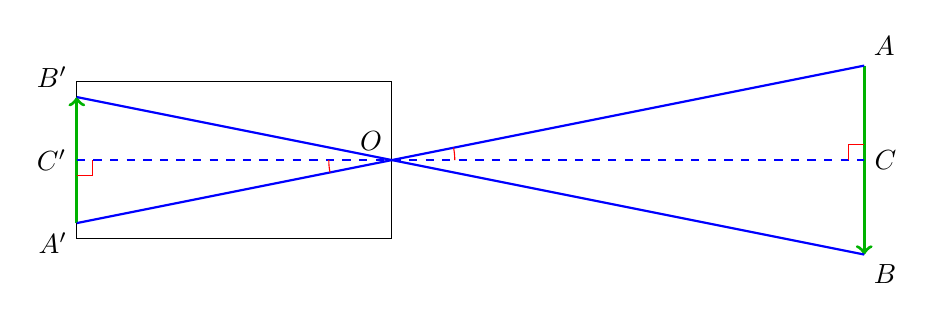
\begin{tikzpicture}
    \draw (-4,-1) rectangle (0, 1);
    \coordinate [label=above left:$O$] (origin) at (0,0);
    \coordinate [label=below left:$A'$] (imga) at (-4, -0.8);
    \coordinate [label=above left:$B'$] (imgb) at (-4, 0.8);
    \draw [->,very thick,green!70!black] (imga) -- (imgb);
    \coordinate [label=above right:$A$] (obja) at (6, 1.2);
    \coordinate [label=below right:$B$] (objb) at (6, -1.2);
    \draw [->,very thick,green!70!black] (obja) -- (objb);

    \draw [thick,blue] (imga) -- (obja);
    \draw [thick,blue] (imgb) -- (objb);

    \coordinate (imgc) at ($0.5*(imga)+0.5*(imgb)$);
    \coordinate (objc) at ($0.5*(obja)+0.5*(objb)$);
    \draw [thick,blue,dashed]  (imgc) node [text=black,anchor=east]  {$C'$} -- (objc) node [text=black,anchor=west]  {$C$};

    % Angle arc towards image
    \begin{scope}
      \clip (imga) -- (origin) -- (imgc) -- cycle;
      \draw [red] (origin) circle (0.8);
    \end{scope}

    % Angle arc towards object
    \begin{scope}
      \clip (obja) -- (origin) -- (objc) -- cycle;
      \draw [red] (origin) circle (0.8);
    \end{scope}

    \draw [red] ($(imgc) + (0.2, 0)$) -- ($(imgc) + (0.2, -0.2)$) -- ($(imgc) + (0.0, -0.2)$);

    \draw [red] ($(objc) + (-0.2, 0)$) -- ($(objc) + (-0.2, 0.2)$) -- ($(objc) + (0.0, 0.2)$);
  \end{tikzpicture}
  \centering
  \begin{align}
    \frac{AC}{OC} &= \frac{A'C'}{OC'}\\
    \frac{\text{Size of object}}{\text{Distance of object}} &= \frac{\text{Size of screen}}{\text{Distance of image}}
  \end{align}
\end{frame}

\begin{comment} % Too complicated
  
\begin{frame}{Exercise}

  Can we compute the distance of object?\\
  \pause
  \begin{align}
    \text{Distance of object} = \frac{\text{Size of object}}{\text{Size of image}} \times \text{Distance of screen}
  \end{align}
\end{frame}

\end{comment}

\begin{frame}{Distance and size of moon.}

  \begin{tikzpicture}
    \node [inner sep=0] (moonsmall) at (-3,0) {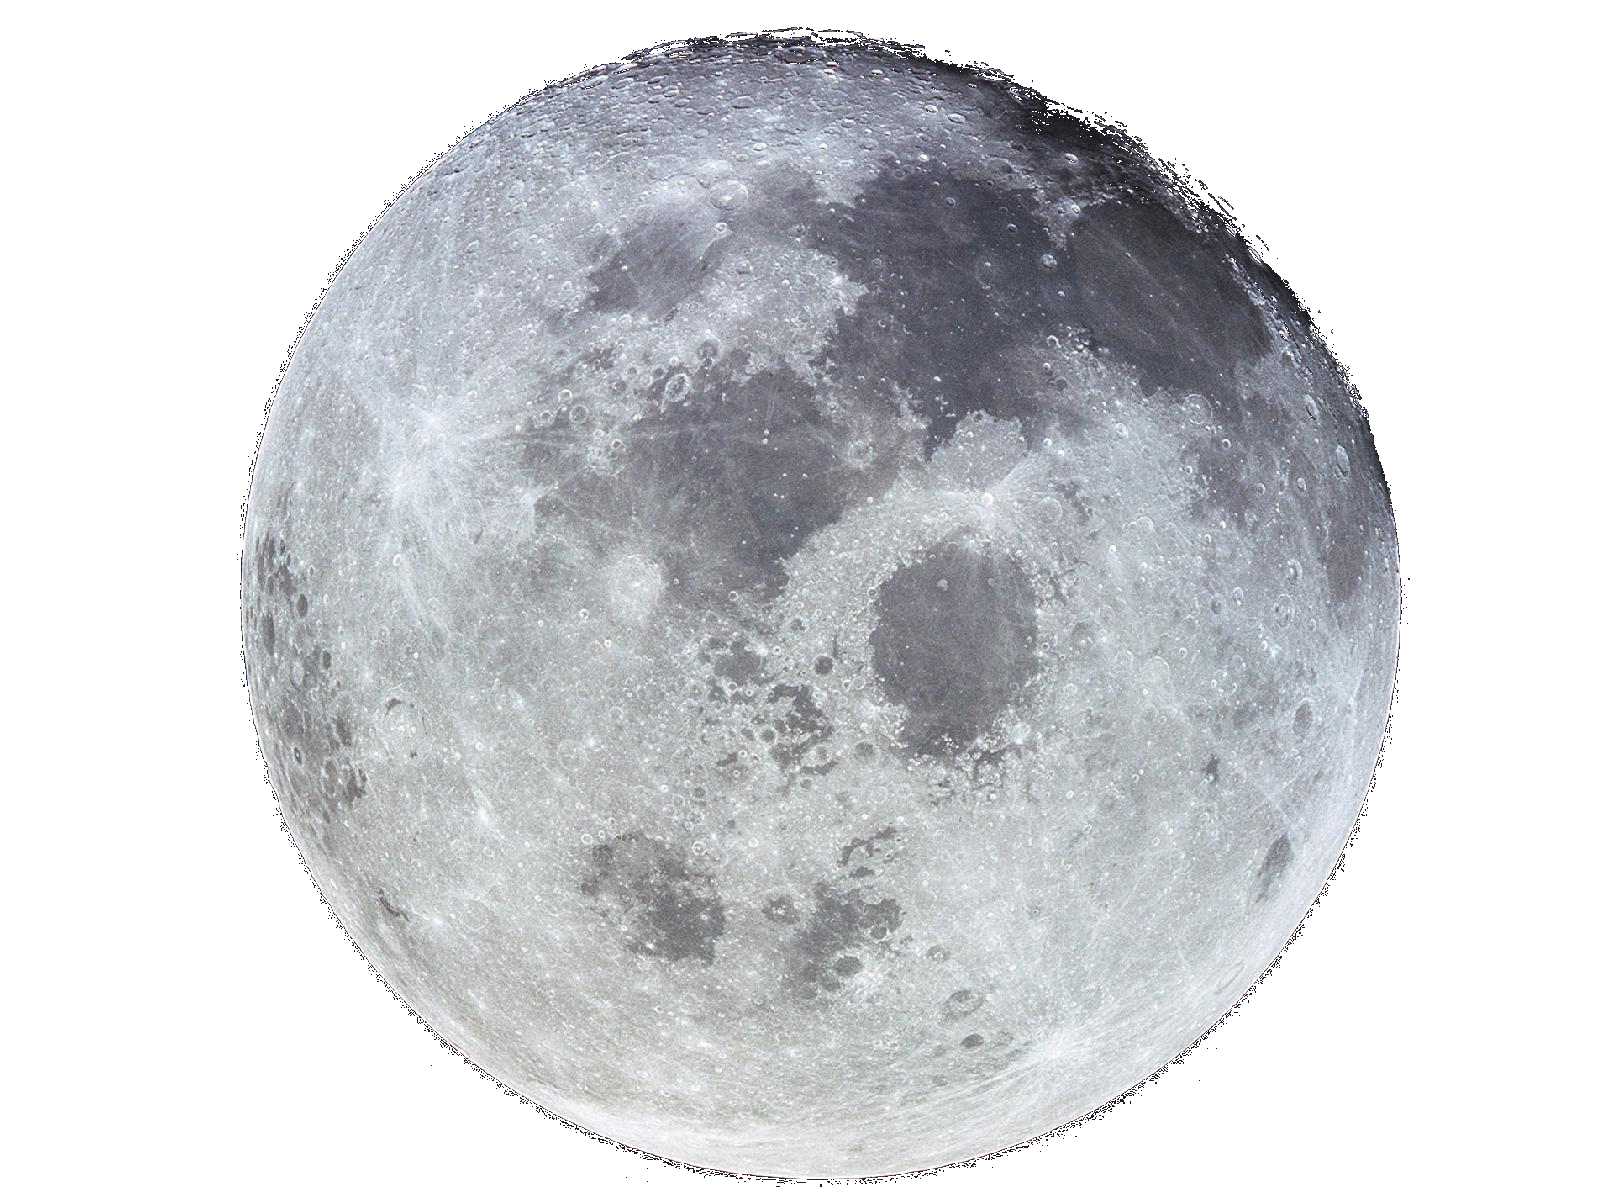
\includegraphics[height=1.5cm]{media/moon.png}};
    \node [inner sep=0] (moonlarge) at (-6,0) {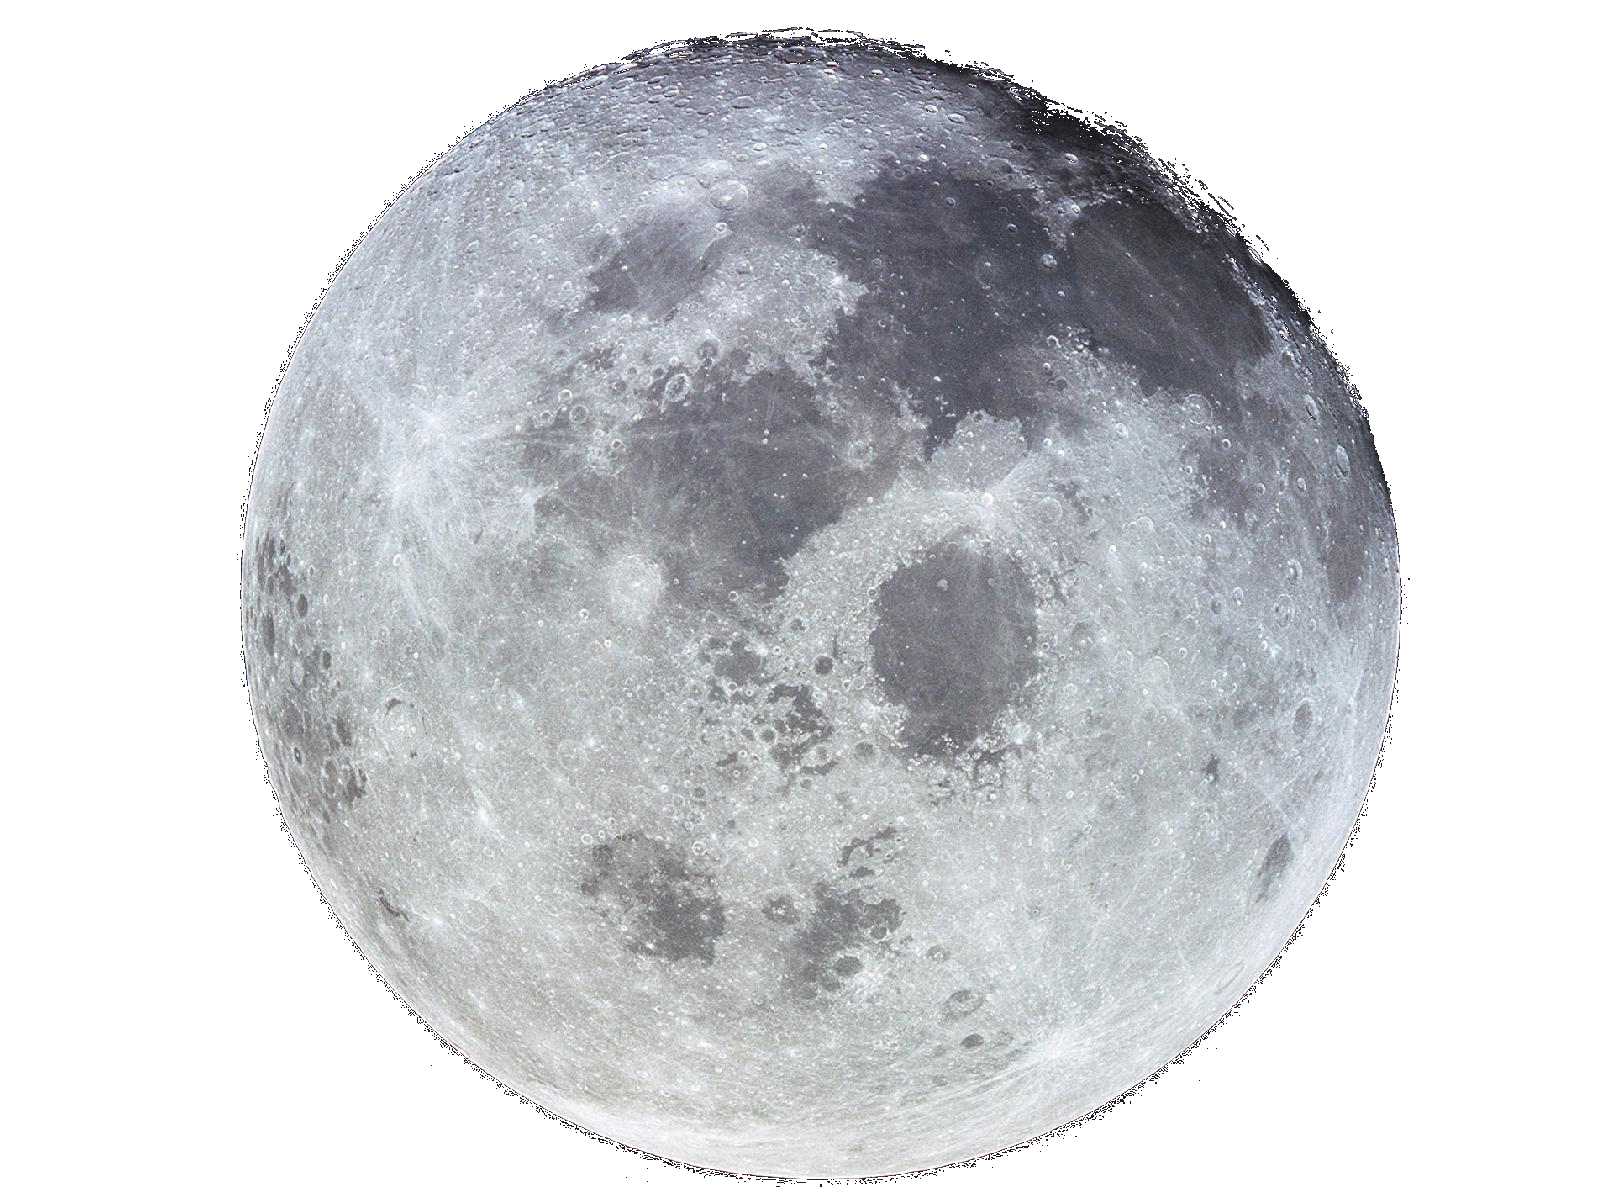
\includegraphics[height=3.0cm]{media/moon.png}};
    \node (eye) at (0,0) {
\includegraphics[height=1cm]{media/eye-left-viewing.png}};
    \draw (0,-1) rectangle (1,1);
    \node [inner sep=0] (moonimg) at (1,0) {\raisebox{\depth}{\scalebox{-1}[-1]{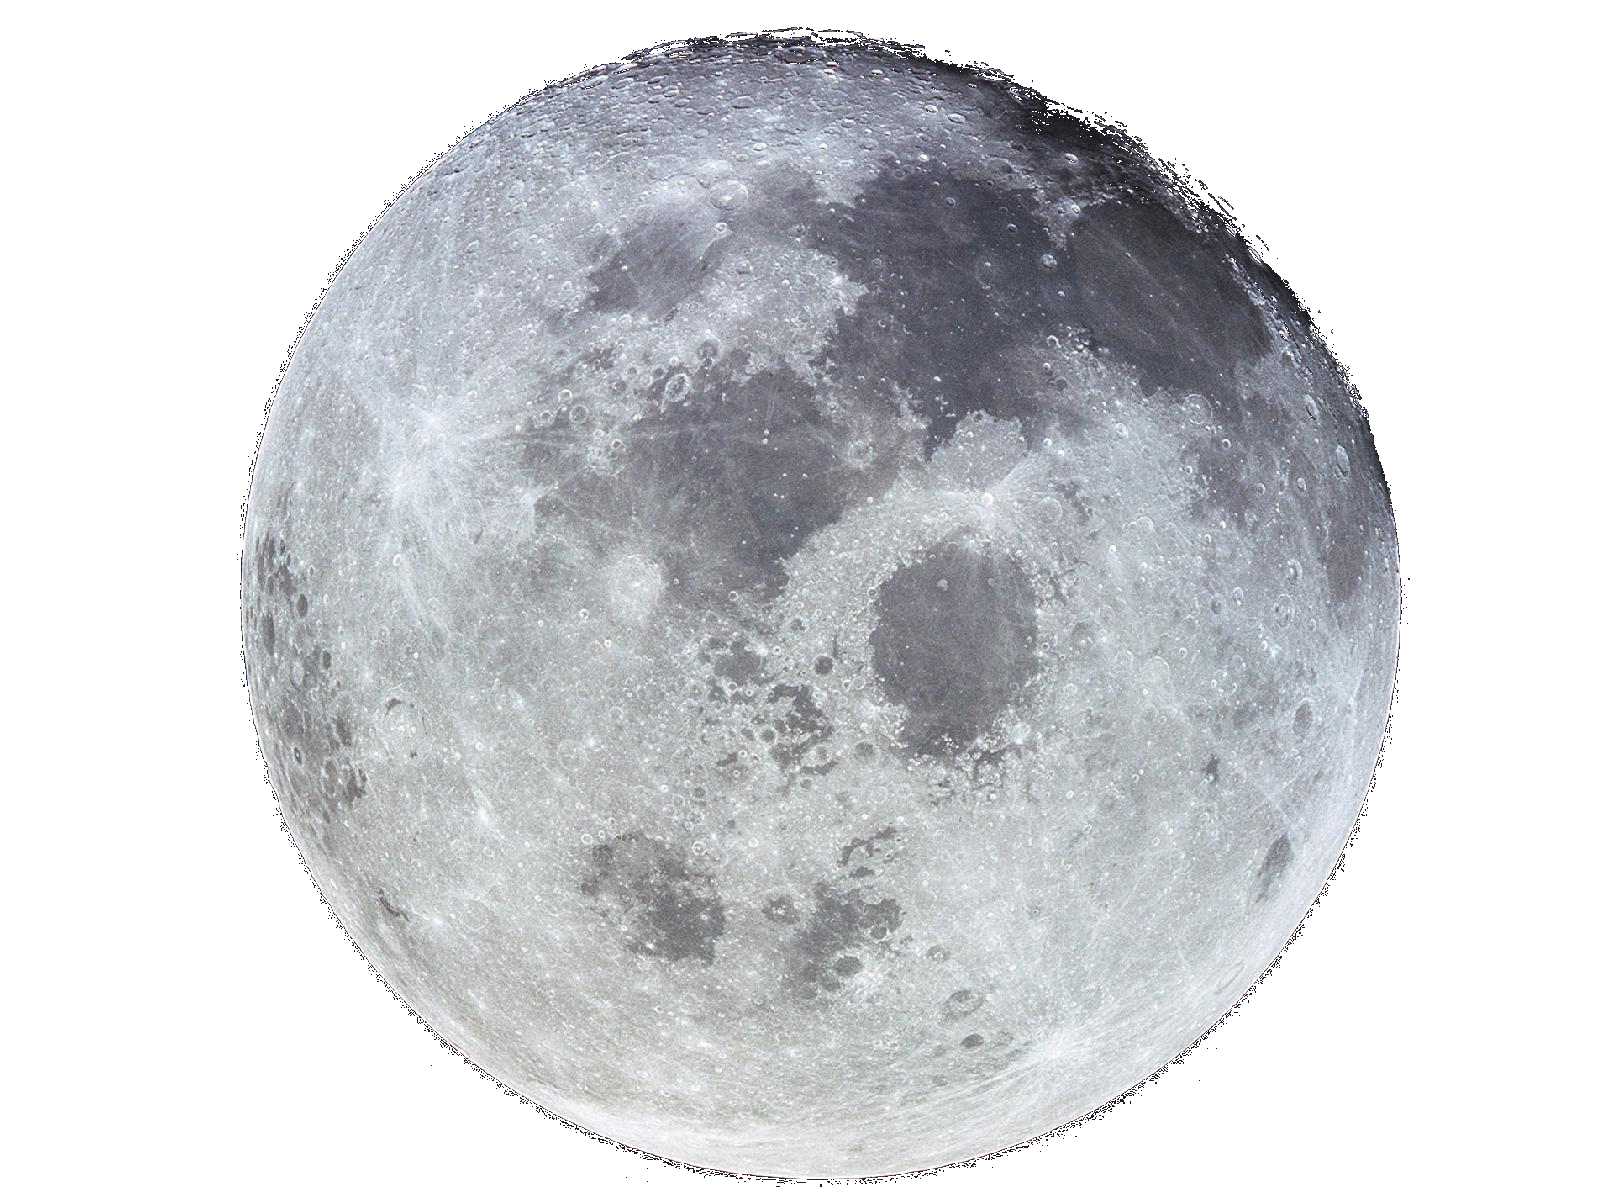
\includegraphics[height=.5cm]{media/moon.png}}}};
    \draw (moonimg.south) -- (moonlarge.north);
    \draw (moonimg.north) -- (moonlarge.south);
  \end{tikzpicture}
  \pause
  \\
  We CANNOT compute both the distance and size of moon from single image.
\end{frame}

\begin{frame}{Effect of changing screen-aperture distance}
  We will now study effect of changing screen-aperture distance on the image.

  Let's cut the cup along the slit.\\
  \hl{TODO:Include a picture for instructions}
\end{frame}

\begin{frame}[fragile]{Scientific method}
  
             \newcommand{\textonecolor}[1]{\ifnum2<#1black\else black!50\fi}
  \only<2>{\renewcommand{\textonecolor}[1]{\ifnum3<##1black\else black!50\fi}}
  \only<4>{\renewcommand{\textonecolor}[1]{\ifnum4<##1black\else black!50\fi}}

             \newcommand{\nodeonecolor}[1]{\if3#1red!20\else none\fi}
  \only<2>{\renewcommand{\nodeonecolor}[1]{\if4##1red!20\else none\fi}}
  \only<4>{\renewcommand{\nodeonecolor}[1]{\if5##1red!20\else none\fi}}
  \begin{center}
    \begin{tikzpicture}[]

      \def \n {6}
      \def \radius {3}
      \def \margin {15} % margin in angles, depends on the radius

      \foreach \s/\t in {1/Purpose,2/Research,3/Hypothesis,4/Experiment,5/Analysis,6/Conclusion}
      {
        \node[fill=\nodeonecolor{\s},text=\textonecolor{\s},circle,minimum width=3] at ({360/\n * (\s - 1)}:\radius) {\t};
        \draw[->, >=latex] ({360/\n * (\s - 1)+\margin}:\radius) 
        arc ({360/\n * (\s - 1)+\margin}:{360/\n * (\s)-\margin}:\radius);
      }
    \end{tikzpicture}
    \addtooverlay<.(3)>{%
      \draw[fill=black,opacity=1.00] 
      (current page.north east) rectangle (current page.south west);
      \node at (current page.center) {
\includegraphics[height=\textheight]{media/tree.png}};
    }
  \end{center}

\end{frame}

\section{Effect of Aperture size}
\begin{frame}{Guess what happens?}
  ... if we make the pinhole a little bigger.\\
  \hl{TODO:Include an image to show how big of a hole}
\end{frame}

\begin{frame}[fragile]{Scientific method}
  
             \newcommand{\textonecolor}[1]{\ifnum2<#1black\else black!50\fi}
  \only<2>{\renewcommand{\textonecolor}[1]{\ifnum3<##1black\else black!50\fi}}
  \only<4>{\renewcommand{\textonecolor}[1]{\ifnum4<##1black\else black!50\fi}}

             \newcommand{\nodeonecolor}[1]{\if3#1red!20\else none\fi}
  \only<2>{\renewcommand{\nodeonecolor}[1]{\if4##1red!20\else none\fi}}
  \only<4>{\renewcommand{\nodeonecolor}[1]{\if5##1red!20\else none\fi}}
  \begin{center}
    \begin{tikzpicture}[]

      \def \n {6}
      \def \radius {3}
      \def \margin {15} % margin in angles, depends on the radius

      \foreach \s/\t in {1/Purpose,2/Research,3/Hypothesis,4/Experiment,5/Analysis,6/Conclusion}
      {
        \node[fill=\nodeonecolor{\s},text=\textonecolor{\s},circle,minimum width=3] at ({360/\n * (\s - 1)}:\radius) {\t};
        \draw[->, >=latex] ({360/\n * (\s - 1)+\margin}:\radius) 
        arc ({360/\n * (\s - 1)+\margin}:{360/\n * (\s)-\margin}:\radius);
      }
    \end{tikzpicture}
    \addtooverlay<.(3)>{%
      \draw[fill=black,opacity=1.00] 
      (current page.north east) rectangle (current page.south west);
      \node at (current page.center) {
\includegraphics[height=\textheight]{media/tree.png}};
    }
  \end{center}

\end{frame}

\begin{frame}{Guess what happens?}
  ... if we make the pinhole a little bigger.\\
  \pause
  {\color{red} Image becomes brighter but blurred}
\end{frame}
\note{Some may observe that the image becomes "clearer". 
This is because of increased brightness. Especially when you are observing the tree. In case of the lamp the "blurrer" observation should be easier.}

\begin{frame}{Why?}
  \usetikzlibrary{calc}
\begin{tikzpicture}
\draw [very thick] (-2,-1) rectangle (0,1);
\fill [white] (-0.1,-0.08) rectangle (0.1,0.08);
\node [inner sep=-10] (tree) at (4,0) {
\includegraphics[height=4cm]{media/tree.png}};
\node [inner sep=-5](treeimg) at (-2,0) {\raisebox{\depth}{\scalebox{-1}[-1]{
\includegraphics[height=2cm]{media/tree.png}}}};
\draw [very thick] ($(tree.south)+(-.5,0.2)$) -- (treeimg.north);
\draw [very thick] ($(tree.north)+(-.5,-0.2)$) -- (treeimg.south);
\end{tikzpicture}
\\
  \usetikzlibrary{calc}
\begin{tikzpicture}
\draw [very thick] (-2,-1) rectangle (0,1);
\fill [white] (-0.1,-0.2) rectangle (0.1,0.2);
\node [inner sep=-10] (tree) at (4,0) {
\includegraphics[height=4cm]{media/tree.png}};
\node [inner sep=-5](treeimg1) at (-2,0.2) {\raisebox{\depth}{\scalebox{-1}[-1]{
\includegraphics[height=2cm]{media/tree.png}}}};
\draw [very thick] ($(tree.south)+(-.5,0.2)$)-- (treeimg1.north);
\draw [very thick] ($(tree.north)+(-.5,-0.2)$) -- (treeimg1.south);


\node [inner sep=-5](treeimg2) at (-2,-0.2) {\raisebox{\depth}{\scalebox{-1}[-1]{
\includegraphics[height=2cm]{media/tree.png}}}};

\draw [very thick] ($(tree.south)+(-.5,0.2)$) -- (treeimg2.north);
\draw [very thick] ($(tree.north)+(-.5,-0.2)$) -- (treeimg2.south);
\end{tikzpicture}

\end{frame}

\begin{frame}{Fun fact!!}
  \begin{center}
    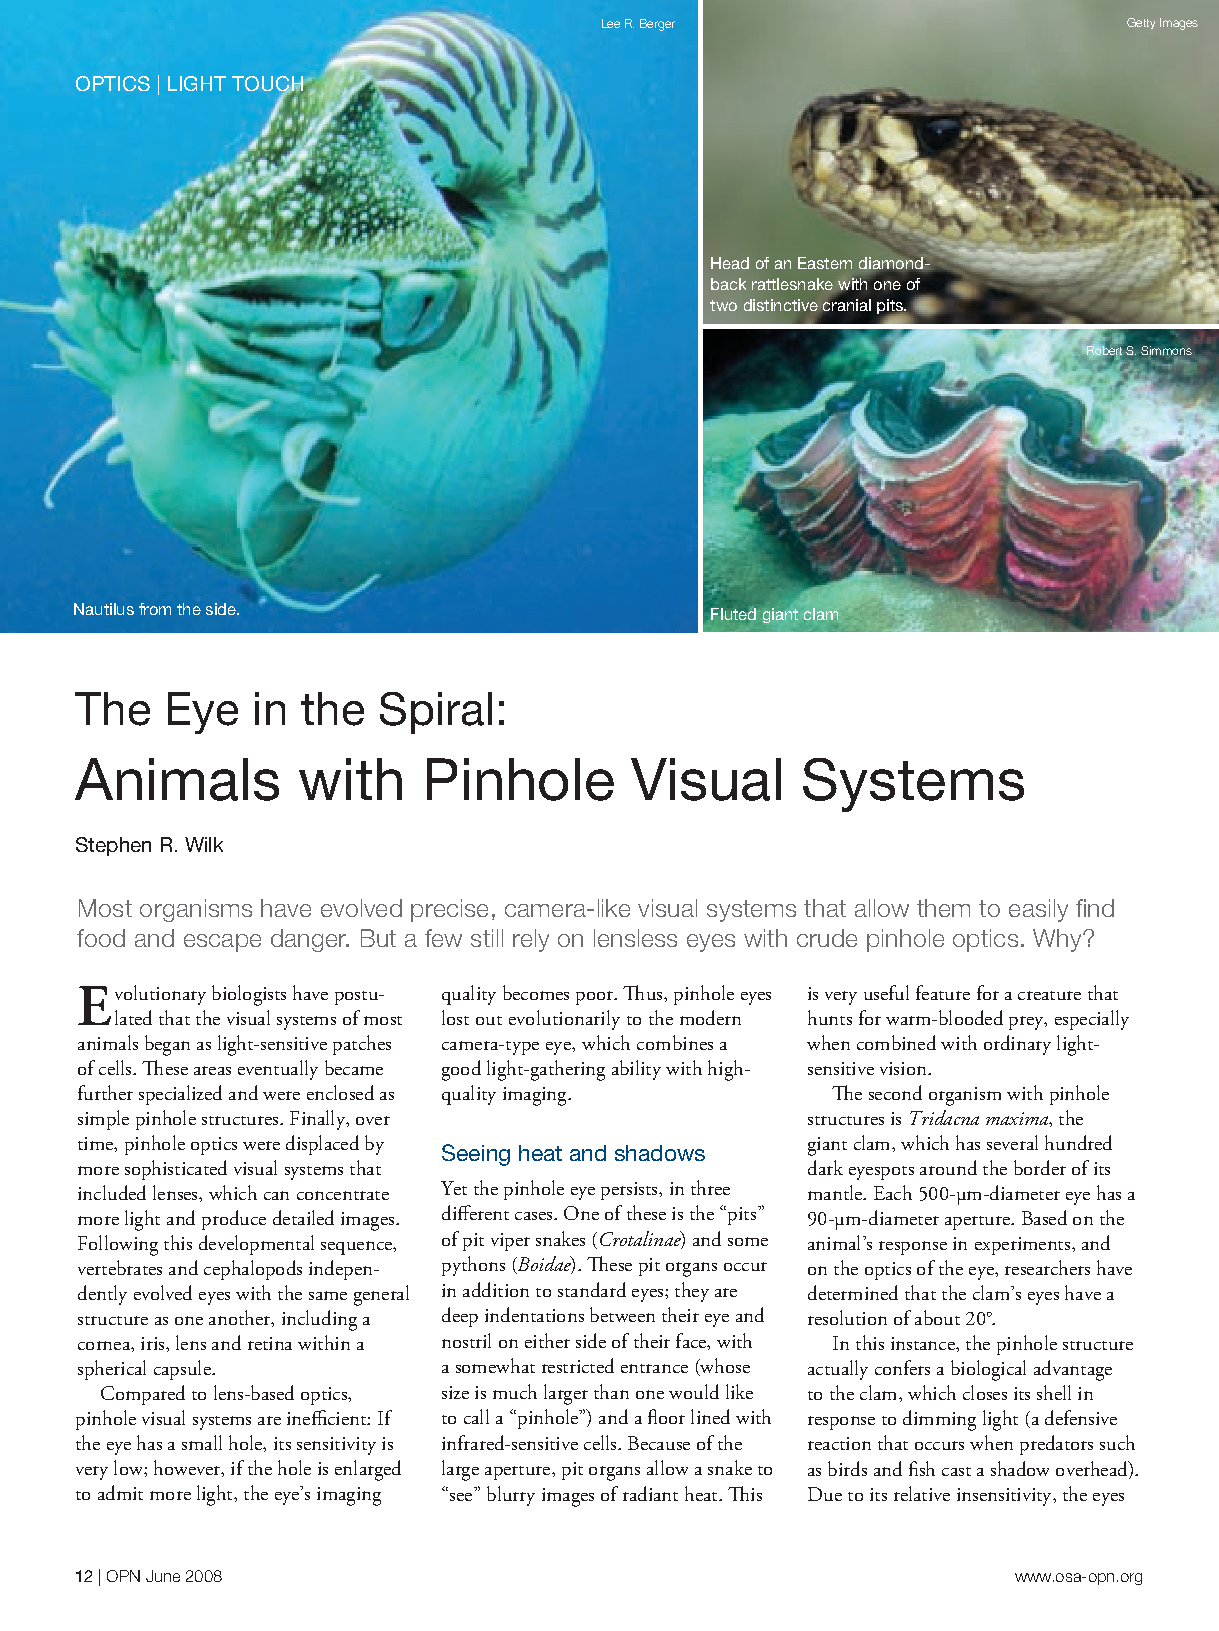
\includegraphics[width=0.8\textwidth, trim=0 5in 0 0,clip]{media/animalspinhole.pdf}
  \end{center}
\end{frame}
\begin{frame}
  \begin{center}
    \includemedia[label=chambered-nautilus-accident,
      width=\linewidth,height=0.6\linewidth, % 16:9
      activate=pageopen,
      addresource=media/chambered-nautilus-accident.mp4,
      flashvars={
        source=media/chambered-nautilus-accident.mp4
        &loop=false             % loop video
        &scaleMode=letterbox   % preserve aspect ratio while scaling the video
      }
    ]{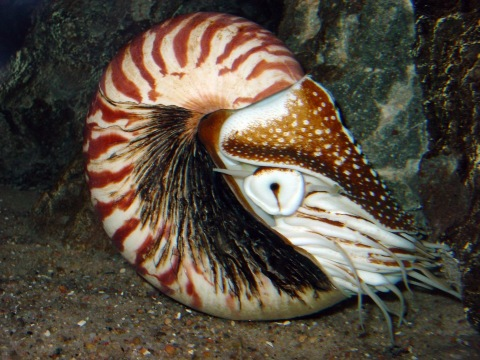
\includegraphics{media/chambered-nautilus-accident.jpg}}{VPlayer.swf}
  \end{center}
\end{frame}

\section{Number of Apertures}
\begin{frame}{Guess what happens}
  ... if we make multiple holes around the pinhole?\\
  \hl{TODO:Include a picture of how many holes}
\end{frame}

\begin{frame}[fragile]{Scientific method}
  
             \newcommand{\textonecolor}[1]{\ifnum2<#1black\else black!50\fi}
  \only<2>{\renewcommand{\textonecolor}[1]{\ifnum3<##1black\else black!50\fi}}
  \only<4>{\renewcommand{\textonecolor}[1]{\ifnum4<##1black\else black!50\fi}}

             \newcommand{\nodeonecolor}[1]{\if3#1red!20\else none\fi}
  \only<2>{\renewcommand{\nodeonecolor}[1]{\if4##1red!20\else none\fi}}
  \only<4>{\renewcommand{\nodeonecolor}[1]{\if5##1red!20\else none\fi}}
  \begin{center}
    \begin{tikzpicture}[]

      \def \n {6}
      \def \radius {3}
      \def \margin {15} % margin in angles, depends on the radius

      \foreach \s/\t in {1/Purpose,2/Research,3/Hypothesis,4/Experiment,5/Analysis,6/Conclusion}
      {
        \node[fill=\nodeonecolor{\s},text=\textonecolor{\s},circle,minimum width=3] at ({360/\n * (\s - 1)}:\radius) {\t};
        \draw[->, >=latex] ({360/\n * (\s - 1)+\margin}:\radius) 
        arc ({360/\n * (\s - 1)+\margin}:{360/\n * (\s)-\margin}:\radius);
      }
    \end{tikzpicture}
    \addtooverlay<.(3)>{%
      \draw[fill=black,opacity=1.00] 
      (current page.north east) rectangle (current page.south west);
      \node at (current page.center) {
\includegraphics[height=\textheight]{media/tree.png}};
    }
  \end{center}

\end{frame}

\begin{frame}{Guess what happens}
  ... if we make multiple holes around the pinhole?\\
  \pause
  {\color{red} Did you get multiple images?}
\end{frame}

\begin{frame}{Evolution of eye}

                \newcommand{\overlayhide}{\fill [rounded corners,white,opacity=0.8] (0,0) -- (0,0.65) --(0.55,0.65) --  (0.55, 1.0) -- (1,1) -- (1,0) -- cycle;}
    \only<2->{\renewcommand{\overlayhide}{\fill [rounded corners,white,opacity=0.8] (0,0) -- (0,0.65) --(0.55,0.65) --  (0.55, 0.65) -- (1,0.65) -- (1,0) -- cycle;}}
    \only<3->{\renewcommand{\overlayhide}{\fill [rounded corners,white,opacity=0.8] (0,0) -- (0,0.33) --(0.50,0.33) --  (0.50, 0.65) -- (1,0.65) -- (1,0) -- cycle;}}
    \only<4->{\renewcommand{\overlayhide}{\fill [rounded corners,white,opacity=0.8] (0,0) -- (0,0.33) --(0.50,0.33) --  (0.50, 0.33) -- (1,0.33) -- (1,0) -- cycle;}}
    \only<5->{\renewcommand{\overlayhide}{\fill [rounded corners,white,opacity=0.8] (0,0) -- (0,0.00) --(0.50,0.00) --  (0.50, 0.33) -- (1,0.33) -- (1,0) -- cycle;}}
    \only<6->{\renewcommand{\overlayhide}{\fill [rounded corners,white,opacity=0.8] (0,0) -- (0,0.00) --(0.50,0.00) --  (0.50, 0.00) -- (1,0.00) -- (1,0) -- cycle;}}
  \begin{center}

    \begin{tikzpicture}
      \node [anchor=south west,inner sep=0](img) at (0,0) {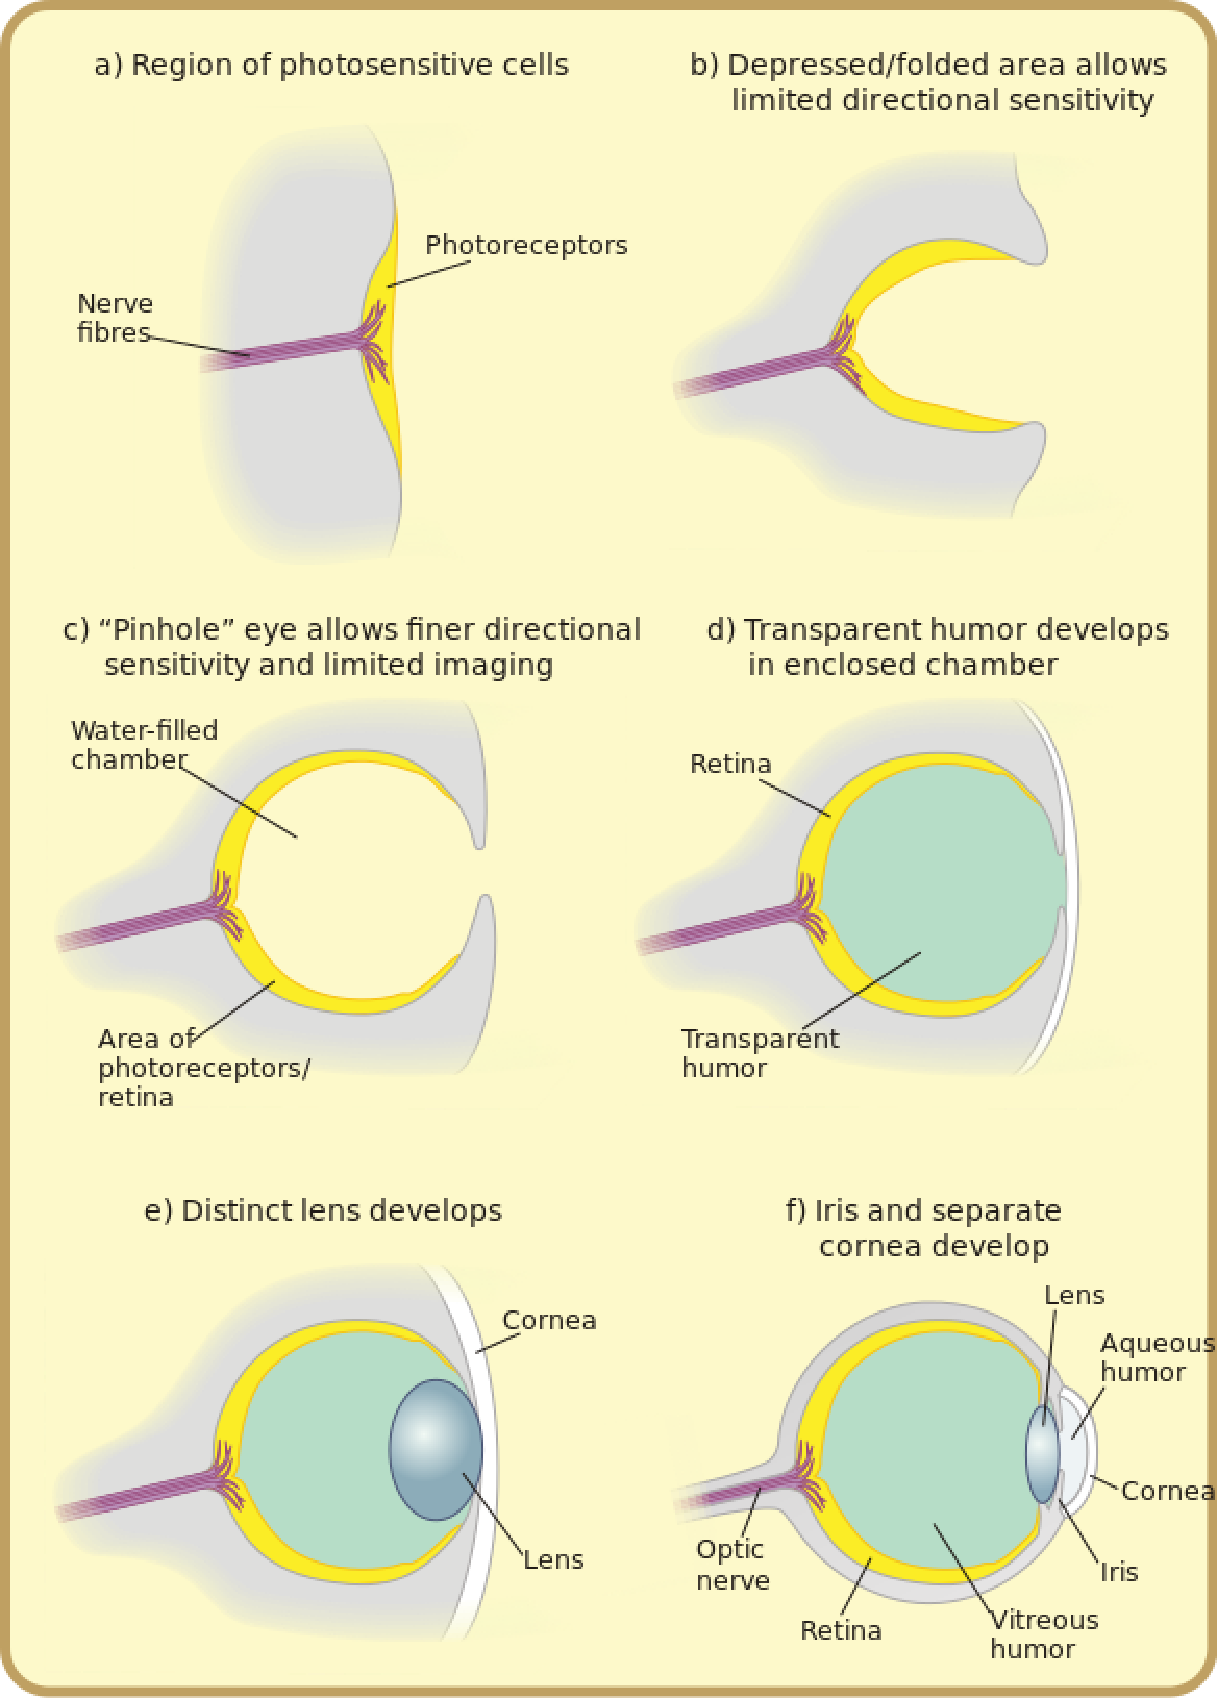
\includegraphics[height=0.8\textheight]{media/Diagram_of_eye_evolution.pdf}};
      \begin{scope}[x={(img.south east)},y={(img.north west)}]
        \overlayhide
      \end{scope}
    \end{tikzpicture}
  \end{center}
\end{frame}

\begin{frame}{Introducing lens}
  We want to find out a lens that will make our camera better.
  \hl{TODO:Include a picture of holding lens (not the right one) with the pinhole camera}
\end{frame}

\note{We give a bunch of lenses to the kids and let them figure out the right lens}

\begin{frame}[fragile]{Scientific method}
  
             \newcommand{\textonecolor}[1]{\ifnum2<#1black\else black!50\fi}
  \only<2>{\renewcommand{\textonecolor}[1]{\ifnum3<##1black\else black!50\fi}}
  \only<4>{\renewcommand{\textonecolor}[1]{\ifnum4<##1black\else black!50\fi}}

             \newcommand{\nodeonecolor}[1]{\if3#1red!20\else none\fi}
  \only<2>{\renewcommand{\nodeonecolor}[1]{\if4##1red!20\else none\fi}}
  \only<4>{\renewcommand{\nodeonecolor}[1]{\if5##1red!20\else none\fi}}
  \begin{center}
    \begin{tikzpicture}[]

      \def \n {6}
      \def \radius {3}
      \def \margin {15} % margin in angles, depends on the radius

      \foreach \s/\t in {1/Purpose,2/Research,3/Hypothesis,4/Experiment,5/Analysis,6/Conclusion}
      {
        \node[fill=\nodeonecolor{\s},text=\textonecolor{\s},circle,minimum width=3] at ({360/\n * (\s - 1)}:\radius) {\t};
        \draw[->, >=latex] ({360/\n * (\s - 1)+\margin}:\radius) 
        arc ({360/\n * (\s - 1)+\margin}:{360/\n * (\s)-\margin}:\radius);
      }
    \end{tikzpicture}
    \addtooverlay<.(3)>{%
      \draw[fill=black,opacity=1.00] 
      (current page.north east) rectangle (current page.south west);
      \node at (current page.center) {
\includegraphics[height=\textheight]{media/tree.png}};
    }
  \end{center}

\end{frame}

\section{Lenses}
\begin{frame}{Introducing lens}
  Add the double convex lens in front of multiple pinholes?\\
  \pause
  Do you see all images merging into one?\\
  What happened?
\end{frame}

\begin{frame}{Understanding refraction}
  \centering
  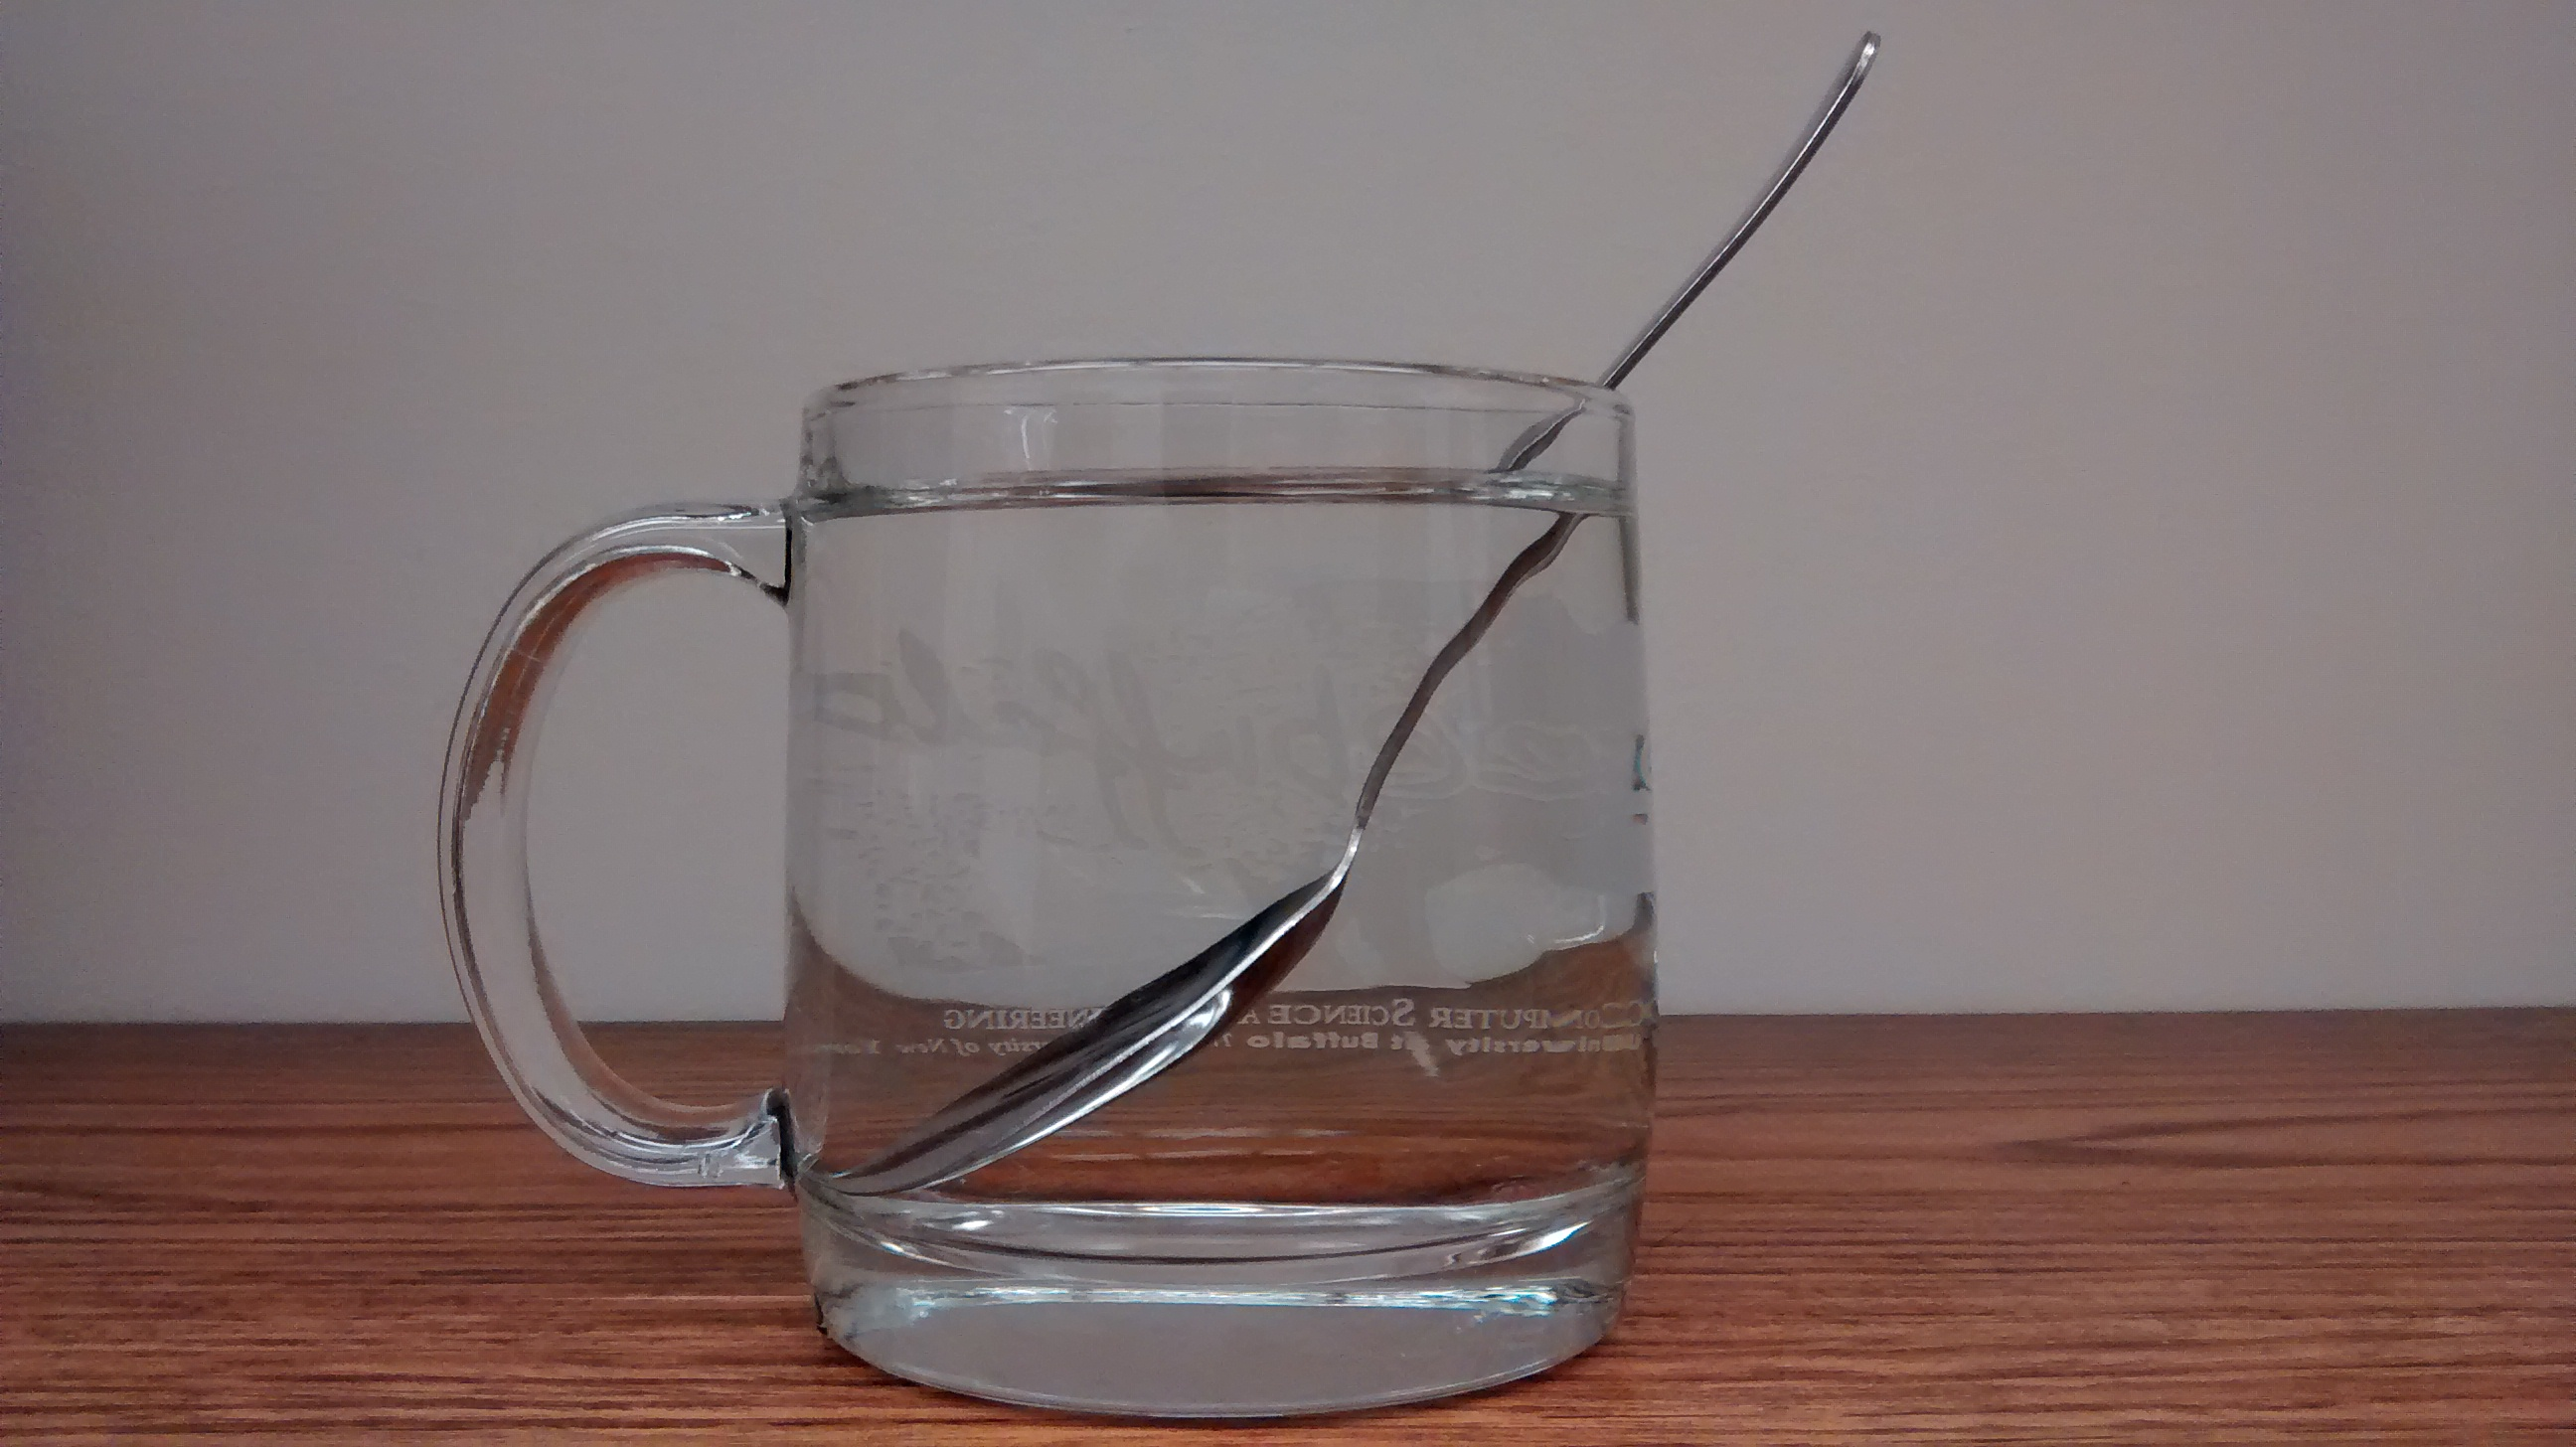
\includegraphics[width=\textwidth]{media/refractionspoon.jpg}
\end{frame}

\begin{frame}{Refraction}
  Light bends towards normal when enters a denser medium \\
  \visible<2->{
  Light bends away from normal when enters a lighter medium}
  \begin{center}
    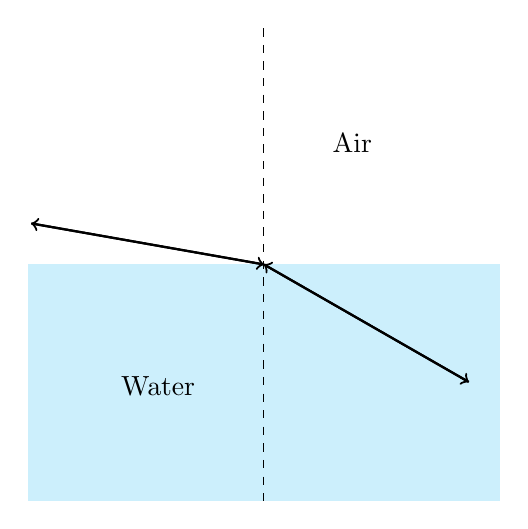
\begin{tikzpicture}[scale=3.0]
      \fill [cyan!20!white] (-1,-1) rectangle (1,0);
      \draw [dashed] (90:1) -- (-90:1);
      \visible<-1>{
        \draw [->,thick] (170:1) -- (0,0);
        \draw [->,thick] (0,0) -- (-29.84:1);
      }
      \visible<2->{
        \draw [<-,thick] (170:1) -- (0,0);
        \draw [<-,thick] (0,0) -- (-29.84:1);
      }
      \node at (60:0.5) [anchor=south west] {Air};
      \node at (-120:0.5) [anchor=north east] {Water};
    \end{tikzpicture}
  \end{center}
\end{frame}

\begin{frame}{Refraction in nature: Twinkling stars}
  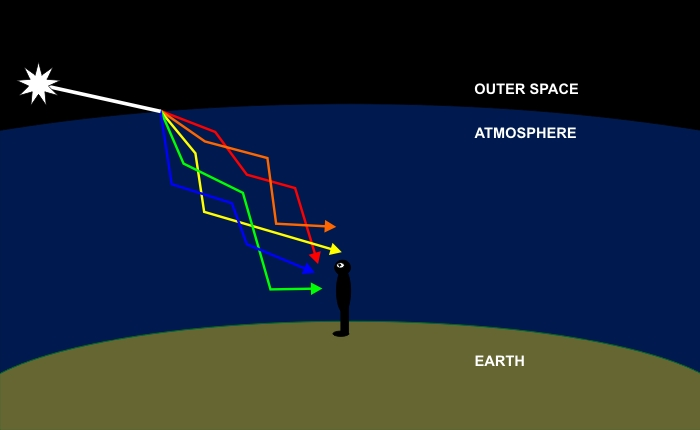
\includegraphics[width=\textwidth]{media/twinkle.jpg}
\end{frame}
\begin{frame}{Refraction in nature: Longer days}
  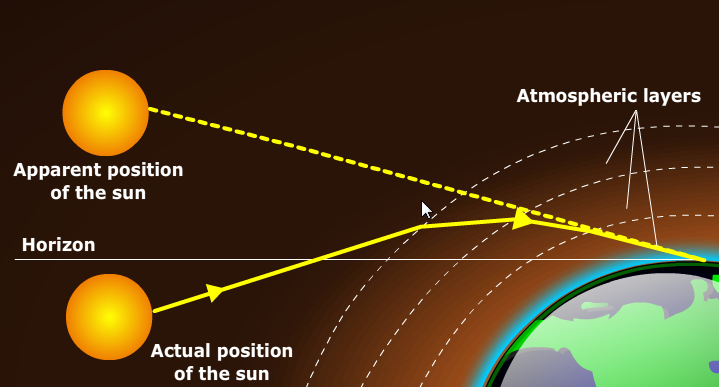
\includegraphics[width=\textwidth]{media/sunset.png}
\end{frame}

\begin{comment} % Too complicated
\begin{frame}{Snell's law}
  \begin{center}
    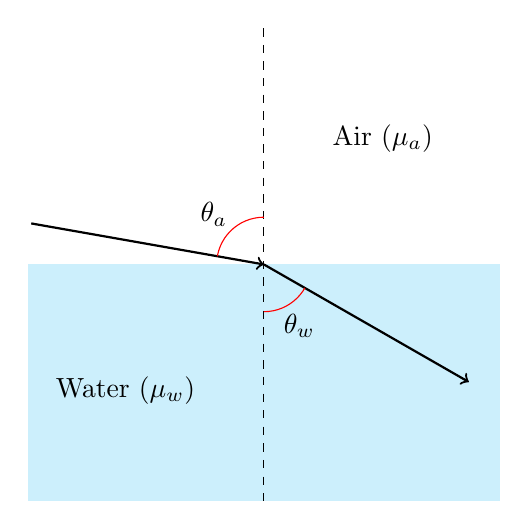
\begin{tikzpicture}[scale=3.0]
      \fill [cyan!20!white] (-1,-1) rectangle (1,0);
      \draw [dashed] (90:1) -- (-90:1);
      \draw [->,thick] (170:1) -- (0,0);
      \draw [->,thick] (0,0) -- (-29.84:1);
      \node at (60:0.5) [anchor=south west] {Air ($\mu_a$)};
      \node at (-120:0.5) [anchor=north east] {Water ($\mu_w$)};
      \begin{scope}
        \clip (0,0) -- (-29.84:1) -- (-90:1) -- cycle;
        \draw [red] (0,0) circle (0.2);
        \node at (-60:0.3) {$\theta_w$};
      \end{scope}
      \begin{scope}
        \clip (0,0) -- (170:1) -- (90:1) -- cycle;
        \draw [red] (0,0) circle (0.2);
        \node at (135:0.3) {$\theta_a$};
      \end{scope}
    \end{tikzpicture}
    \begin{align*}
      \frac{\sin \theta_a }{\sin \theta_w} &= \frac{\mu_w }{\mu_a}
    \end{align*}
  \end{center}
\end{frame}
\end{comment}

\begin{frame}[fragile]{Snell's law}
  \begin{center}
    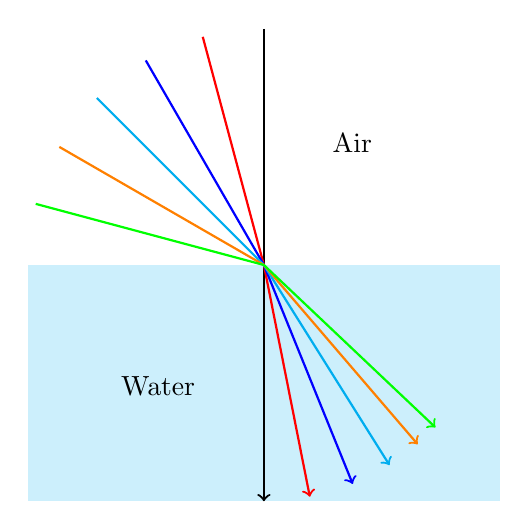
\begin{tikzpicture}[scale=3.0]
      \fill [cyan!20!white] (-1,-1) rectangle (1,0);
      \foreach \s/\c in {0/black,1/red,2/blue, 3/cyan, 4/orange, 5/green} 
      {
        \pgfmathsetmacro{\aw}{asin(sin(15*\s)/1.33)}

        \draw [->,thick,\c] (90+15*\s:1) -- (0,0) -- ({-90+\aw}:1);
      }
      \node at (60:0.5) [anchor=south west] {Air};
      \node at (-120:0.5) [anchor=north east] {Water};
    \end{tikzpicture}
  \end{center}
\end{frame}

\begin{frame}{Refraction at lens}
  \begin{tikzpicture} 
    \def\r{6}
    \coordinate (fp) at (-5.0,0);


    \begin{scope} 
      \clip (0,-4) rectangle (2,4);
      \draw [fill=cyan!20,name path=lensright,very thick] (fp) circle (\r);
    \end{scope}

    \draw [name path=normrightup,thick,dash pattern=on \pgflinewidth off 2pt]($(fp)+(20:0.9*\r)$) -- ($(fp)+ (20:1.1*\r)$);
    \draw [name path=normrightdown,thick,dash pattern=on \pgflinewidth off 2pt]($(fp)+(-20:0.9*\r)$) -- ($(fp)+ (-20:1.1*\r)$);

    \begin{scope} 
      \clip (0,-4) rectangle (-2,4);
      \draw  [fill=cyan!20,name path=lensleft,very thick] ($-1*(fp)$) circle (\r);
    \end{scope}

    \draw [name path=normleftdown,thick,dash pattern=on \pgflinewidth off 2pt]($-1*(fp)+(24:-0.9*\r)$) -- ($-1*(fp)+ (24:-1.1*\r)$);
    \draw [name path=normleftup,thick,dash pattern=on \pgflinewidth off 2pt]($-1*(fp)+(-24:-0.9*\r)$) -- ($-1*(fp)+ (-24:-1.1*\r)$);

    \draw ($-1*(fp)$) -- (fp);

    \path [name intersections={of = lensleft and normleftup}];
    \coordinate (A)  at (intersection-1);
    \draw [thick,<-,stealth-] (A) -- ($(A) + (-3,0)$);

    \path [name intersections={of = lensleft and normleftdown}];
    \coordinate (B)  at (intersection-1);
    \draw [thick,stealth-] (B) -- ($(B) + (-3,0)$);

    \pause
    \path [name intersections={of = lensright and normrightup}];
    \coordinate (Ar)  at (intersection-1);
    \draw [thick,-stealth] (A) -- (Ar);

    \path [name intersections={of = lensright and normrightdown}];
    \coordinate (Br)  at (intersection-1);
    \draw [thick,<-,stealth-] (Br) -- (B);

    \pause
    \draw [thick,-stealth] (Br) -- ($-0.5*(fp)$);
    \draw [thick,-stealth] (Ar) -- ($-0.5*(fp)$);

    \fill ($-0.5*(fp)$) circle (0.1); 
    \node [anchor=north west]at ($-0.5*(fp)$) {Focal Point};

    \pause
    \node [anchor=north east]at ($0.5*(fp)$) {Principal Axis};

    \pause
    \fill (0,0) circle (0.1); 
    \node [anchor=south west] at (0,0) {Optical Center};


  \end{tikzpicture}
\end{frame}

\begin{frame}{Rules by which you can draw ray diagrams}
  \begin{itemize}
    \item Rays parallel to Principal axis converge to the focal point.
    \item Rays passing through optical center do not change direction.
  \end{itemize}
\end{frame}

\begin{frame}{Example}
  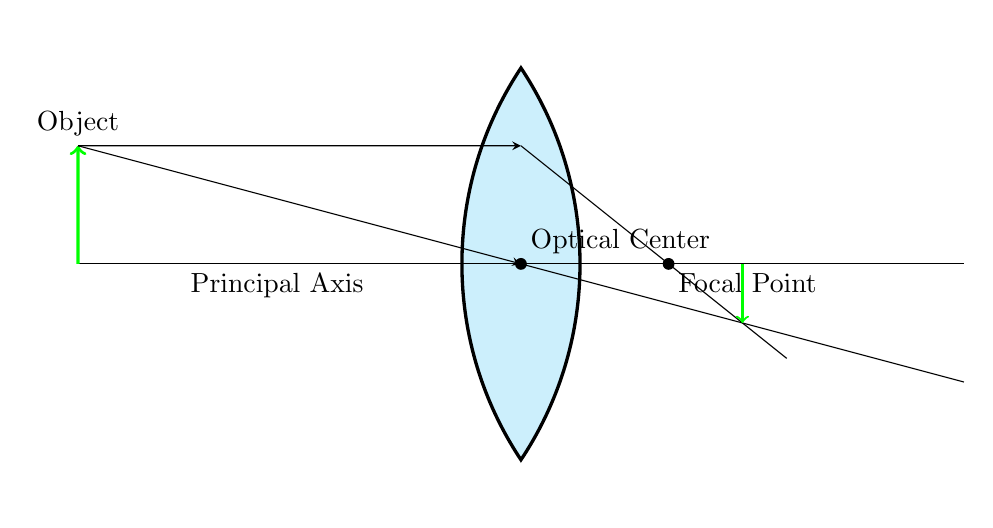
\begin{tikzpicture}[scale=0.75]
    \def\r{6}
    \coordinate (fp) at (-5.0,0);


    \begin{scope} 
      \clip (0,-4) rectangle (2,4);
      \draw [fill=cyan!20,name path=lensright,very thick] (fp) circle (\r);
    \end{scope}

    \begin{scope} 
      \clip (0,-4) rectangle (-2,4);
      \draw  [fill=cyan!20,name path=lensleft,very thick] ($-1*(fp)$) circle (\r);
    \end{scope}

    \draw [name path=principalaxis]($-1.5*(fp)$) -- ($1.5*(fp)$);

    \coordinate [label={above:Object}] (obj) at ($1.5*(fp)+(0,2)$);
    \draw [green,very thick,->] ($1.5*(fp)$) -- (obj);



    \fill ($-0.5*(fp)$) circle (0.1); 
    \only<-1>{\node [anchor=north west]at ($-0.5*(fp)$) {Focal Point};

      \node [anchor=north east]at ($0.5*(fp)$) {Principal Axis};

    \node [anchor=south west] at (0,0) {Optical Center};}
    \fill (0,0) circle (0.1); 

    \pause
    \draw [-stealth] (obj) -- (0,0);
    \draw [-stealth] (obj) -- (0,2);
    \pause
    \draw [name path=ray1] (0,0) -- ($-1.5*(fp)+(0,-2)$);
    \draw [name path=ray2] (0,2) -- ($-0.5*(fp)$) -- ($-1.8*0.5*(fp)-0.8*(0,2)$);
    \path [name path=objray,name intersections={of=ray1 and ray2}](intersection-1) -- ($(intersection-1) + (0,2)$);
    \coordinate (objimg) at (intersection-1);
    \draw [green,thick,<-,name intersections={of=objray and principalaxis}] (objimg) -- (intersection-1);
  \end{tikzpicture}
\end{frame}

\begin{frame}{Interactive animation}
  \url{http://www.pbslearningmedia.org/resource/lsps07.sci.phys.energy.geometoptics/geometric-optics/}
\end{frame}

\newcommand{\includevideo}[1]{
    \includemedia[label=#1,
      width=\linewidth,height=0.6\linewidth, % 16:9
      activate=pageopen,
      addresource=media/#1.mp4,
      flashvars={
        source=media/#1.mp4
        &loop=false             % loop video
        &scaleMode=letterbox   % preserve aspect ratio while scaling the video
      }
    ]{}{VPlayer.swf}
}

\begin{comment} % Not required
\begin{frame}{History of Photography}
  \includevideo{history-of-photography}
\end{frame}

\begin{frame}{Film cameras}
  \includevideo{how-film-cameras-work}
\end{frame}

\begin{frame}{Digital cameras}
  \includevideo{how-digital-cameras-work}
\end{frame}
\end{comment}

\begin{frame}{Questions to think about}
  \begin{itemize}
    \item What is colored light?
    \item Why do we see things in color?
    \item How is rainbow formed?
  \end{itemize}
\end{frame}
\begin{frame}{Sources}
\nocite{bbc2006light}
\nocite{wilk2008eye}
\bibliography{pinhole}
\end{frame}
\bibliographystyle{plain}
\end{document}
